\documentclass[xcolor=svgnames]{beamer}
\usecolortheme[named=blue]{structure}
\usetheme{theme1}
\usepackage{bm}
\usepackage{amsmath}
\usepackage{amssymb}
\usepackage{amsthm}
\usepackage{graphicx}
\usepackage{xcolor}
\usepackage{mathrsfs}
\usepackage{ragged2e}
\usepackage{calc}
\usepackage{tikz}
\usepackage[T1]{fontenc}
\usepackage[firstinits=true,backend=bibtex,bibstyle=numeric-comp,citestyle=authoryear-icomp]{biblatex}
\DeclareCiteCommand{\putCitation}[\mkbibfootnote]
	{\usebibmacro{prenote}}
	{\tiny{
	\printnames[citeauthor]{author}
	\setunit{\addcomma\space}
	\ifentrytype{book}{\printfield{title}}{\printfield[citeield]{shortjournal}}
	(\printfield[citeyear]{year})
	}}
	{\multicitedelim}
	{\usebibmacro{postnote}
}
\DeclareRobustCommand{\abinitio}[0]{\emph{ab initio}}
\DeclareRobustCommand{\Abinitio}[0]{\emph{Ab initio}}
\DeclareRobustCommand{\AbInitio}[0]{\emph{Ab Initio}} % for references
\DeclareRobustCommand{\Schrodinger}[0]{Schr\"{o}dinger}
\DeclareRobustCommand{\Sim}[0]{$\sim$}
\DeclareRobustCommand{\PESs}[0]{PES\,s}
\DeclareRobustCommand{\mc}[1]{\mathcal{#1}}
\DeclareRobustCommand{\mbf}[1]{{\boldsymbol {#1}}}
\addbibresource{masterReferences.bib}
\addtobeamertemplate{frame begin}{}{\justifying}
\title{Quantum Virial Coefficients via Path Integral Monte Carlo: Theory and Development of Novel Algorithms}
\author{PhD dissertation defense by: Ramachandran Subramanian}
\institute[UB]{
\large{Committee: Prof. David A. Kofke (Chair),\\
Prof. Jeffrey R. Errington, Prof. Johannes Hachmann, Dr. Andrew J. Schultz
}}
\date{May 9, 2016}


\AtBeginSection[]
{
\begin{frame}
\frametitle{Overview}
\tableofcontents[currentsection]
\end{frame}
}


\begin{document}
\setbeamertemplate{caption}{\raggedright\insertcaption\par}
	{
	\setbeamertemplate{headline}{}
	\setbeamertemplate{footline}{}
	\begin{frame}
		\titlepage
	\end{frame}
	}
	
	\iffalse
	\begin{frame}
		\frametitle{Overview}
		\tableofcontents
	\end{frame}
	\fi
	
	\section{Introduction}
	\subsection{Virial coefficients}
		\begin{frame}
			\frametitle{Virial equation of state (VEOS)}
                \begin{block}{}
                    \color{blue}{
                    \begin{equation*}
                        \frac{P}{\rho kT} = 1 + B_2(T) \rho + B_3(T) \rho^2 + \ldots
                    \end{equation*}}
                \end{block}
			\begin{itemize}
				\justifying
				\item $B_n$ - $n^{th}$ order virial coefficient represents the effect of interaction of $n$ molecules.
				\item Second and third order virial coefficients are given by:
                \begin{equation*}
                    \begin{aligned}
                        B_2(T) &= -\frac{1}{2} \displaystyle\int d1 ~ f(0,1)\\
                        B_3(T) &= -\frac{1}{3} \displaystyle\int \int d1~d2~f(0,1)~f(0,2)~f(1,2)
                    \end{aligned}
                \end{equation*}
                where $f(0,1) = \Big( \exp \big[ -\beta U_2(\mbf{r}) \big] - 1 \Big) $ and indices `1' and `2' denote the position and orientational degrees of freedom of molecules 1 and 2, respectively, with respect to molecule `0' at the origin.
			\end{itemize}
		\end{frame}

		\begin{frame}
            \frametitle{Main uses:}
			\begin{itemize}
				\justifying
				\item To compute other thermodynamic properties like the Joule-Thomson coefficient, critical point etc.
                \item To rank different potential models by comparing their virial coefficients to experimental results
				\begin{figure}
				\centering
				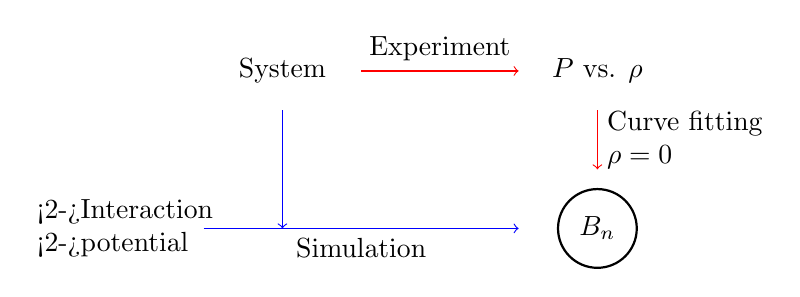
\begin{tikzpicture}
				\node at (-2,3) {System};
				\draw[->,red] (-1,3) -- (1,3);
				\node[above] at (0,3) {Experiment};
				\node at (2,3) {$P$ vs. $\rho$};
				\draw[->,red] (2,2.5) --(2,2.125) node[align=left,right,black]{Curve fitting\\ $\rho = 0$ } -- (2,1.75);
				\node at (2,1) {$B_n$};
				\draw[thick] (2,1) circle [radius=0.5];
				\node[align=left] at (-4,1) {\alert<2->{Interaction}\\ \alert<2->{potential}};
				\draw[->,blue] (-3,1) -- (-1,1) node[below,black] {Simulation} -- (1,1);
				\draw[->,blue] (-2,2.5) -- (-2,1);
				\end{tikzpicture}
				\end{figure}
            \item \visible<2->{To systematically tune and improve potentials as a result.}
			\end{itemize}
		\end{frame}
		
		\begin{frame}
			\frametitle{Empirical potential models}
			\begin{itemize}
				\justifying
				\item Usually functions fitted to experimental data of bulk property measurement.
				\item Represent the net effect of a variety of phenomena taking place including 2 body interactions, multi-body interactions, nuclear quantum effects etc.
				\item As a result, fail to accurately represent interaction potential.
				\item Interaction potentials that better represent condensed (high density) phase fail to predict accurate virial coefficients for the gas (low density) phase.
			\end{itemize}
		\end{frame}
		
		\begin{frame}
			\frametitle{Example - different empirical models of water}
            \begin{itemize}
                \item Importance of the accuracy of interaction potential\putCitation{Benjamin2007}:
            \end{itemize}
            \begin{figure}
            \centering
            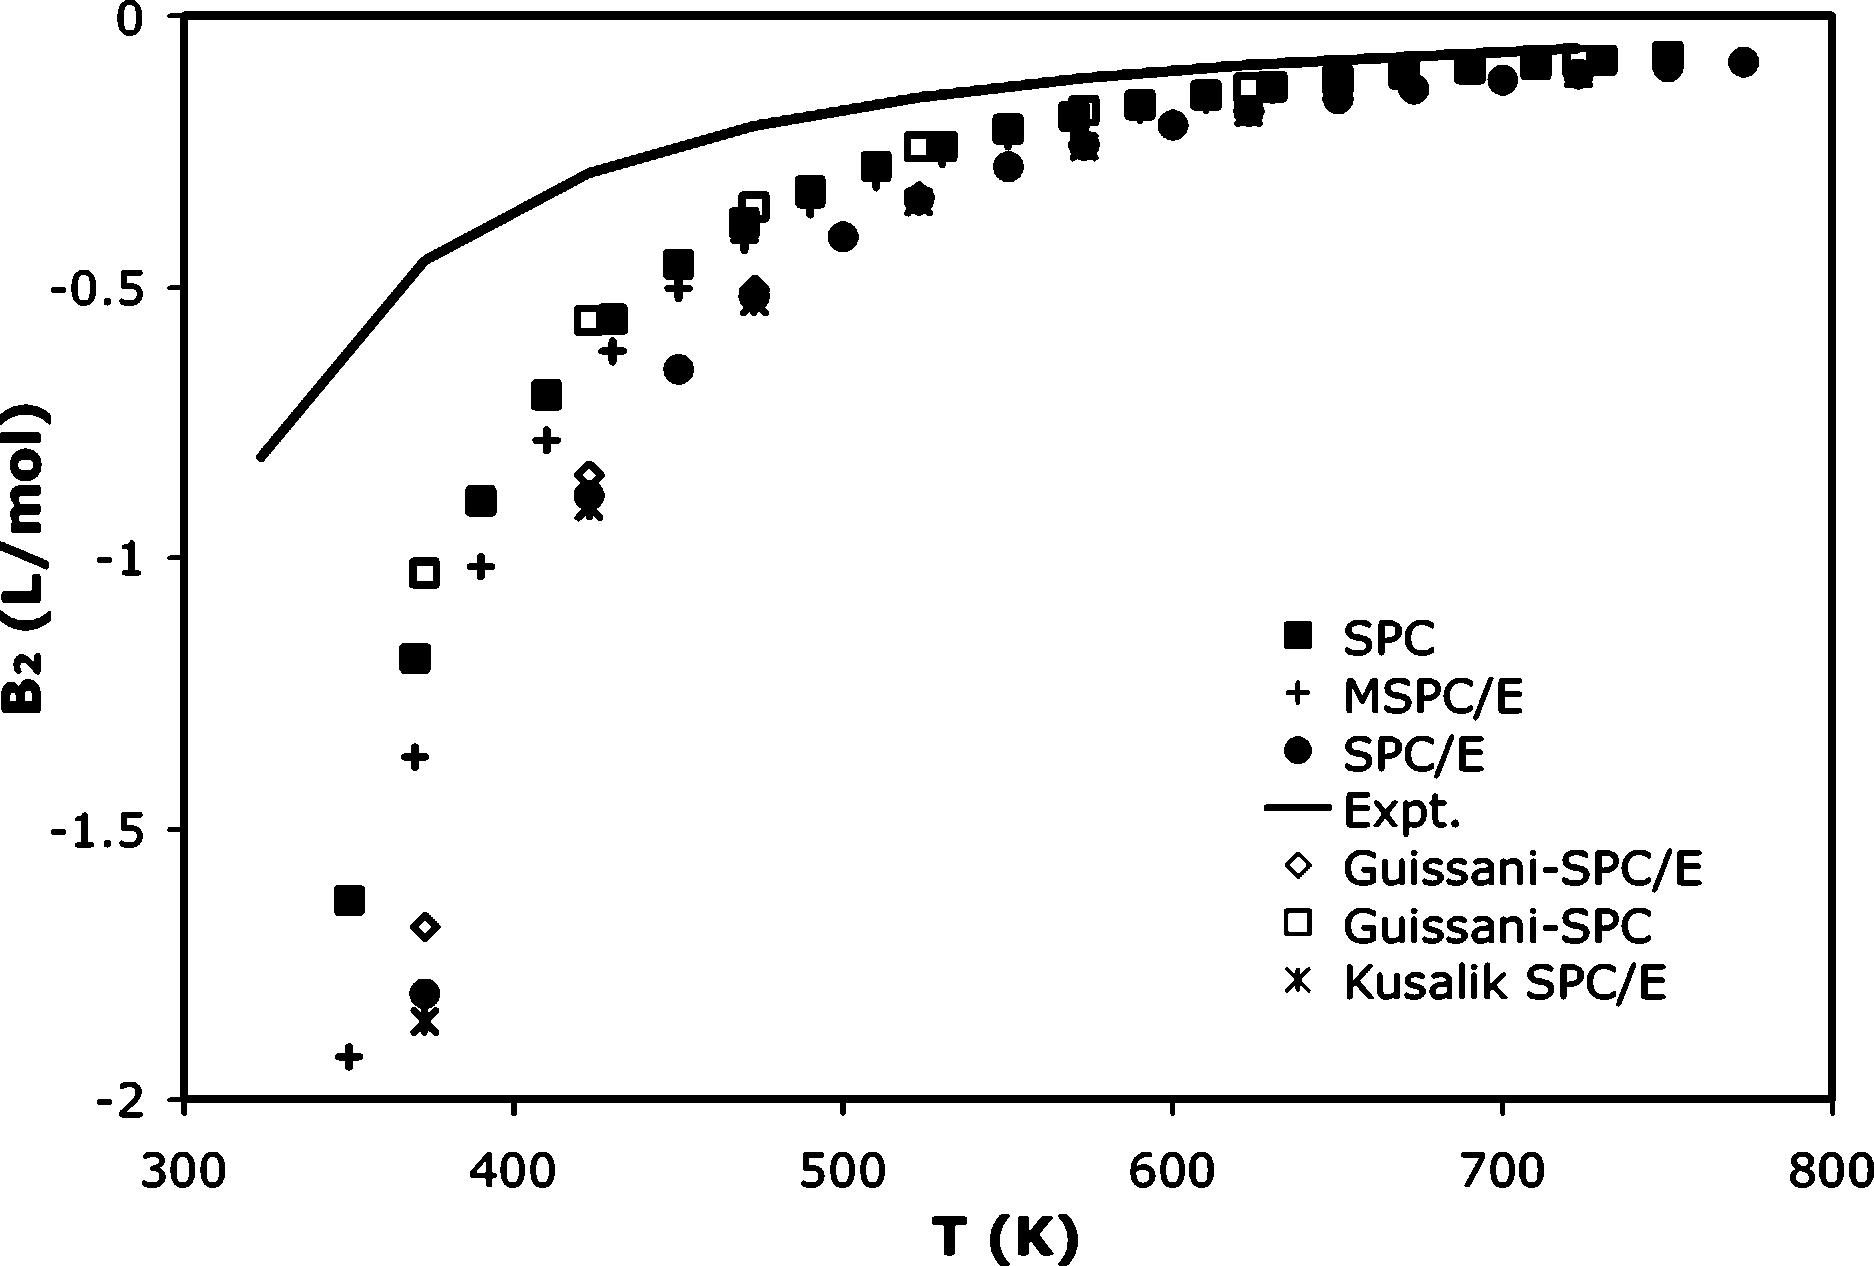
\includegraphics[scale=0.08,keepaspectratio]{ben2a.png}
            \end{figure}
		\end{frame}
    \subsection{\Abinitio{} potentials}
        \begin{frame}
        \frametitle{\Abinitio{} potential models}
            \begin{itemize}
                \item Fundamentally different from empirical models as they focus only on two or three molecules at a time
                \item Solve for the interaction energies starting with the \Schrodinger{} equation and involve many approximations:
                \begin{equation*}
                    \begin{aligned}
                        \mc{H}~\Psi &= E~\Psi, \\
                        \mc{H} &= \mc{T}_e + \mc{T}_N + \mc{V}_{ee} + \mc{V}_{eN} + \mc{V}_{NN}
                    \end{aligned}
                \end{equation*}
                \item Account for electronic structure using different levels of theory and different basis sets
                \item We use potentials fitted to \abinitio{} data rather than compute it on-the-fly (expensive)
            \end{itemize}
            \end{frame}

        \begin{frame}
            \frametitle{Nuclear quantum effects}
            \begin{itemize}
                \justifying
                \item Can be explained by the zero-point vibrational energy and result in uncertainty in the positions of atoms at low temperatures.
                \item Have to be explicitly included in virial coefficient calculations as they are ignored in the development of \abinitio{} potentials.
                \item Semi-classical routes to include quantum effects:
                    \begin{enumerate}
                        \item Computing first order quantum corrections.
                        \item Using an effective potential like the Quadratic Feynman-Hibbs (QFH)\putCitation{Feynman} or Takahashi-Imada (TI)\putCitation{Takahashi1984,Schenter2002}.
                    \end{enumerate}
                \item Quantum route: path integral Monte Carlo (PIMC) (will be explained in detail later).
            \end{itemize}
        \end{frame}
        \begin{frame}
            \frametitle{Nuclear quantum effects}
            \begin{itemize}
                \item Importance of nuclear quantum effects\putCitation{Shaul2012} for helium-4.
            \end{itemize}
            \begin{figure}
            \centering
            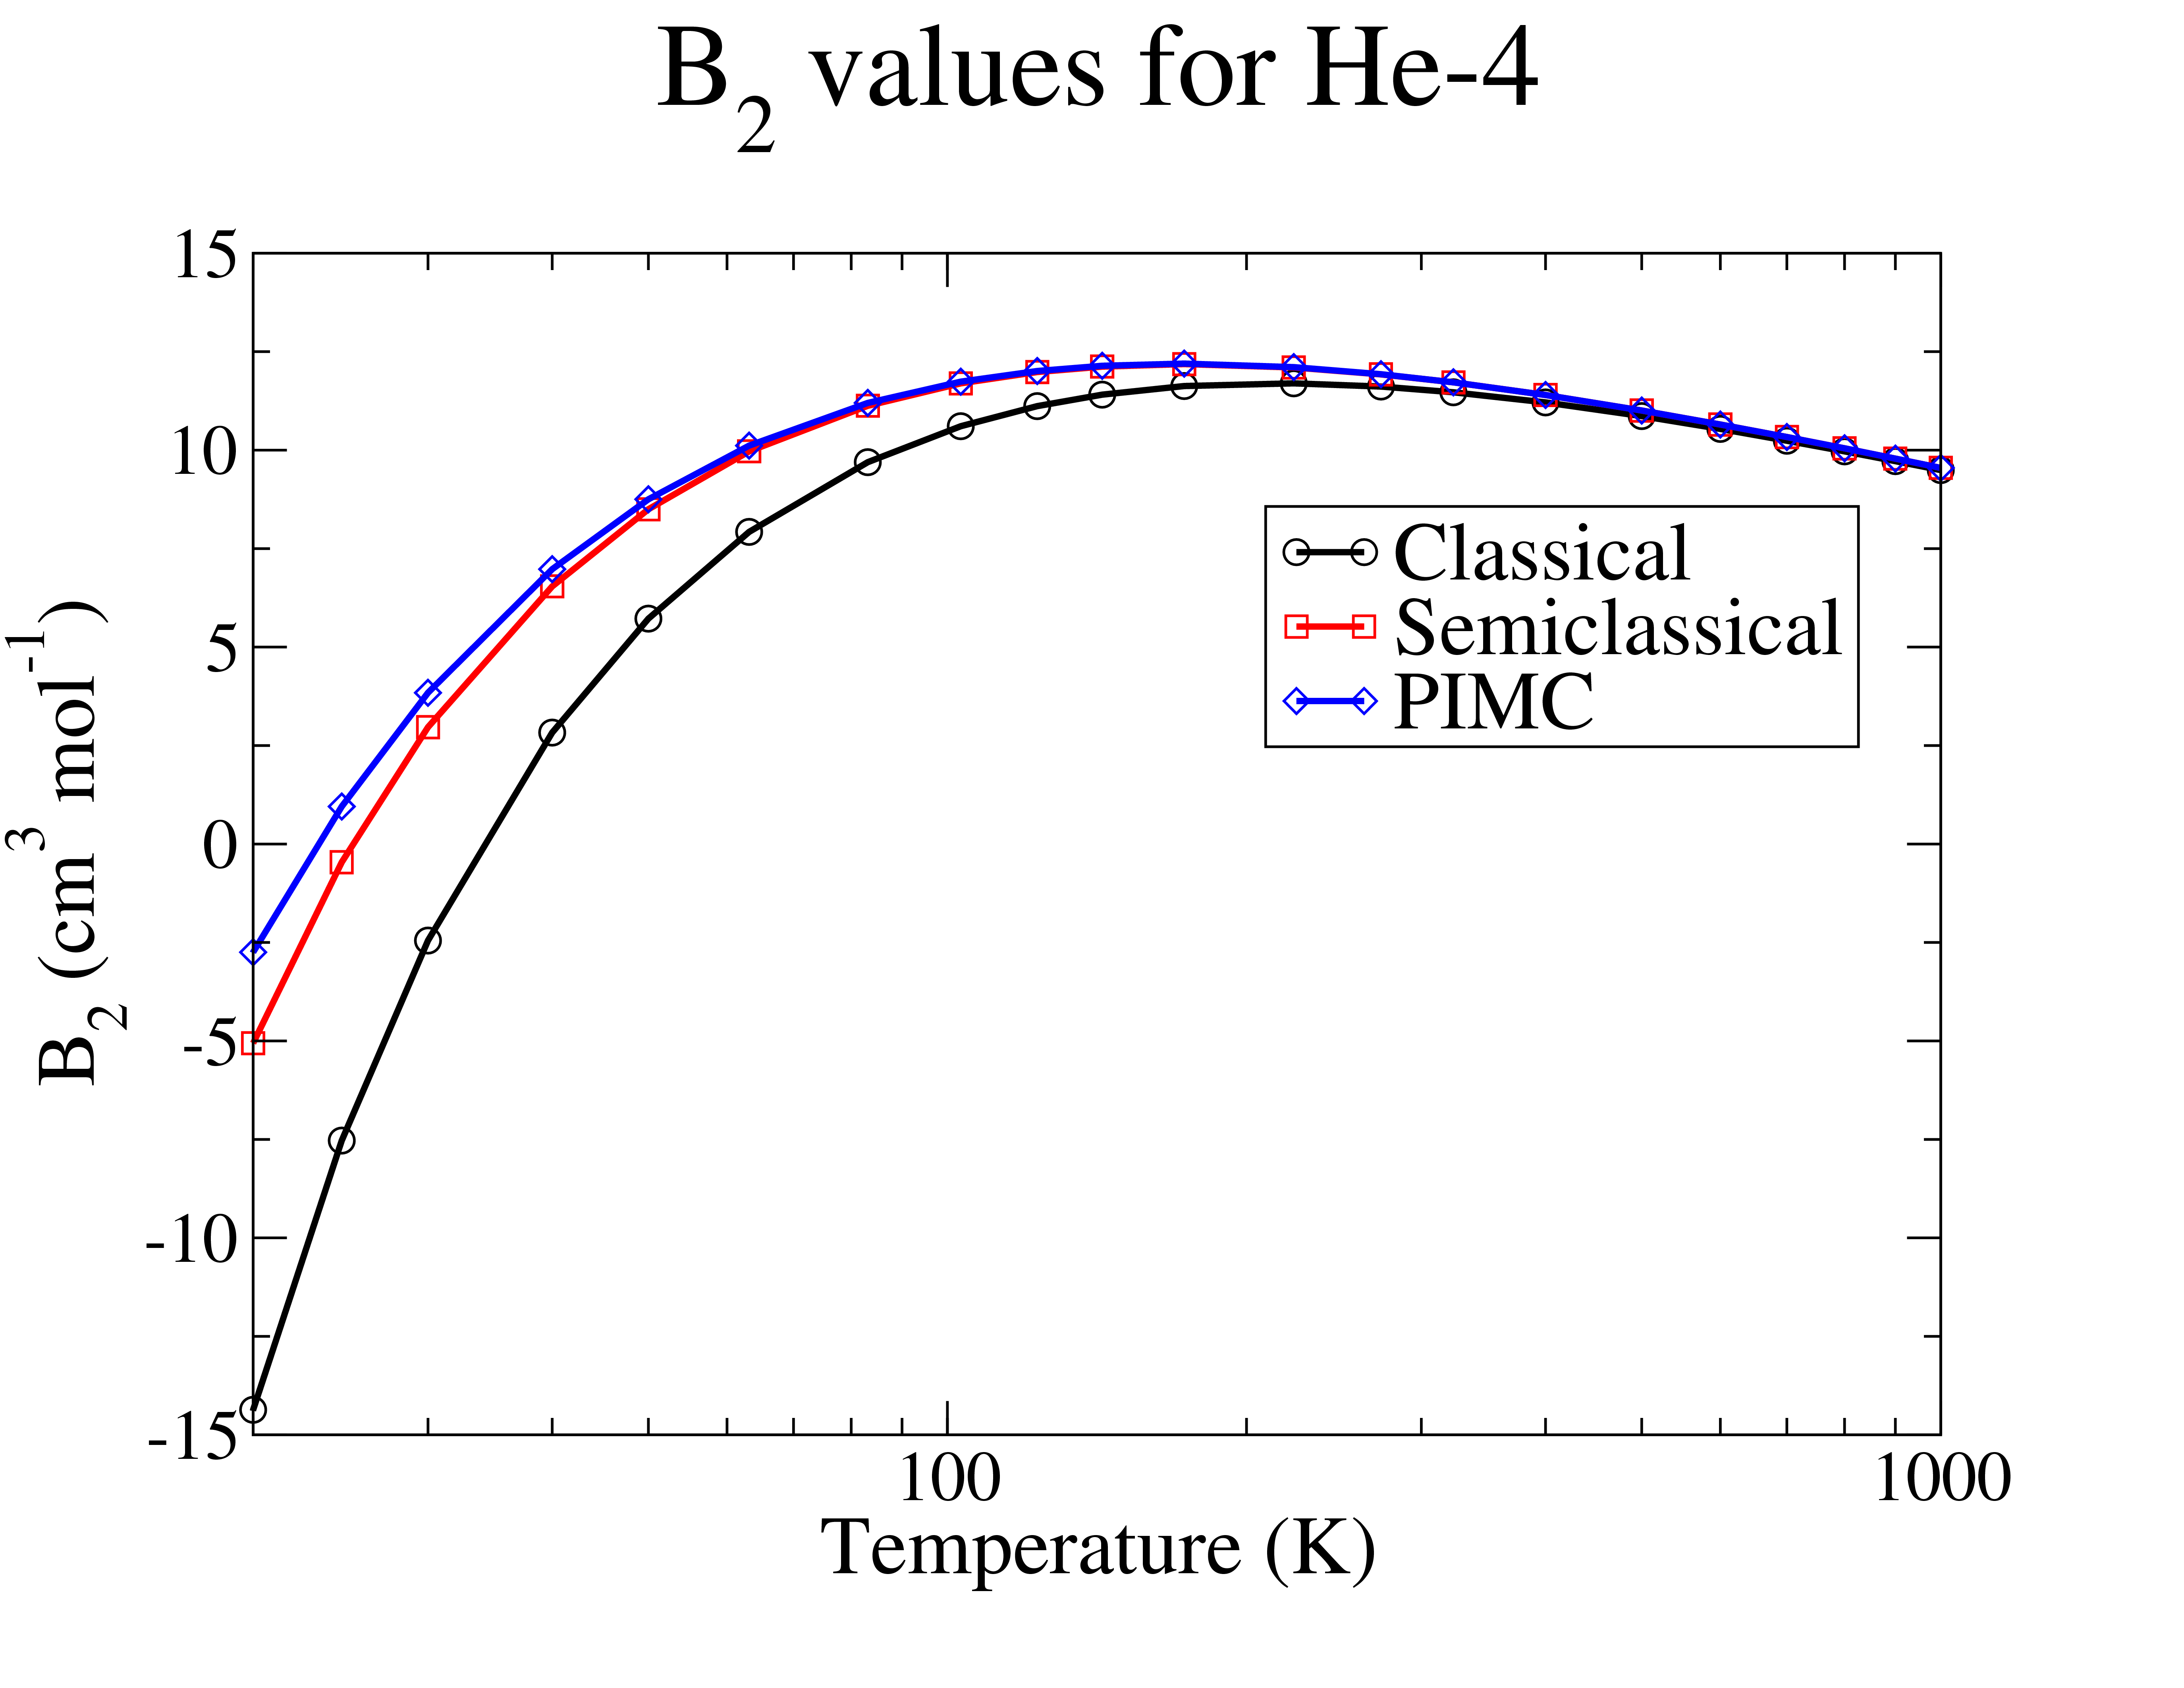
\includegraphics[scale=0.17,keepaspectratio]{B2-Kate.png}
            \end{figure}
        \end{frame}
	
    \section{Objectives}
        \begin{frame}
            \frametitle{Objective}
            \begin{block}{Previous work}
                Monatomic molecules (helium-4 by Kate)
            \end{block}
            \begin{block}{Current challenges}
                \alert<2->{Diatomic molecules: compute accurate virial coefficients using state-of-the-art \abinitio{} potentials and PIMC method.}
            \end{block}
            \begin{block}{Future goals}
                Multiatomic molecules: compute accurate virial coefficients using state-of-the-art \abinitio{} potentials and PIMC method.
            \end{block}
        \end{frame}
	\section{Methods}
	\subsection{Mayer Sampling Monte Carlo}
        \begin{frame}
            \frametitle{Mayer Sampling Monte Carlo}
            \begin{itemize}
            \justifying
                \item Quick recap of the VEOS:
                \begin{equation*}
                    \frac{P}{\rho kT} = 1 + B_2(T) \rho + B_3(T) \rho^2 + \ldots
                \end{equation*}
                \item The number of integrals to be summed\putCitation{Hansen} is: 3 for B$_4$, 10 for B$_5$, 56 for B$_6$, 468 for B$_7$.
                \item MSMC\putCitation{Singh2004} is a free energy perturbation technique to evaluate the integrals in the above equations efficiently.
                \begin{equation*}
                    \label{eq:MSMCworking}
                    \begin{aligned}
                        \Gamma (T) &= \Gamma_o \frac{{<\gamma/\pi>}_\pi / {<\gamma_{os}/\pi>}_\pi}{{<\gamma_o/\pi_o>}_{\pi_o} / {<\gamma_{os}/\pi_o>}_{\pi_o}}\\
                        \gamma_{os} &= \frac{|\gamma_o||\gamma|}{\alpha |\gamma_o| + |\gamma|}
                    \end{aligned}
                \end{equation*}
            \end{itemize}
        \end{frame}
	\subsection{Path Integral Monte Carlo}
        \begin{frame}
            \frametitle{PIMC - thermal density matrix}
            \begin{itemize}
                \justifying
                \item From statistical mechanics: the partition function is given as:
                \begin{equation*}
                    \begin{aligned}
                        P(x) &= \frac{1}{Z} \rho(x,x),\\
                        Z &= \int \rho(x,x) dx \equiv \text{trace} \{\rho\}.
                    \end{aligned}
                \end{equation*}
                \item For the more general case: the probability of going from a state $x$ to $x'$ is proportional to $\rho (x, x'; \beta)$.
                \item Richard Feynman\putCitation{Feynman} was able to connect it with quantum mechanics:
                \begin{equation*}\label{eq:rho}
                    \rho (R , R' ; \beta) = \alert<2>{< R | e^{- \beta \mc{H} } | R' >}
                \end{equation*}
                where $R = \{\bm{r}_1, \bm{r}_2, \ldots \bm{r}_n\}$
            \end{itemize}
        \end{frame}
        \begin{frame}
            \frametitle{Important equations}
            \begin{itemize}
                \justifying
                \item Product of two or more density matrices is also a density matrix\putCitation{Ceperley1995}:
                \begin{align*}\label{eq:convolution}
                    \rho (R_0, R_P; \beta) &= \displaystyle\int \cdots \int dR_1 \, dR_2 \, \ldots \, dR_{P-1} \: \rho (R_0, R_1; \beta/P)\\
                    &\qquad \rho (R_1, R_2; \beta/P) \ldots \rho (R_{P-1}, R_P; \beta/P)
                \end{align*}
                \visible<2->{\item The ``primitive approximation'' is given by\putCitation{Cui1997}:
                \begin{equation*}\label{eq:primitiveApprox}
                    e^{- \frac{\beta}{P} (\mc{T} + \mc{V})} \approx e^{- \frac{\beta}{P} \mc{T}} e^{- \frac{\beta}{P} \mc{V}}
                \end{equation*}
                    }
                \visible<3->{
                \item The Trotter formula\putCitation{Cui1997}:
                \begin{equation*}\label{eq:trotter}
                    e^{- \beta (\mc{T} + \mc{V})} = \lim_{P \to \infty} \Big[ e^{- \frac{\beta}{P} \mc{T}} e^{- \frac{\beta}{P} \mc{V}} \Big]^P
                \end{equation*}
                    }
            \end{itemize}
        \end{frame}
        \begin{frame}
            \frametitle{PIMC}
            \begin{itemize}
                \item More the $P$, the finer the mapping of the quantum mechanical partition function onto the classical ring polymer.
            \end{itemize}
            \begin{center}
                \begin{overlayarea}{8cm}{2cm}
                    \begin{figure}[H]
                        \only<1>{
                        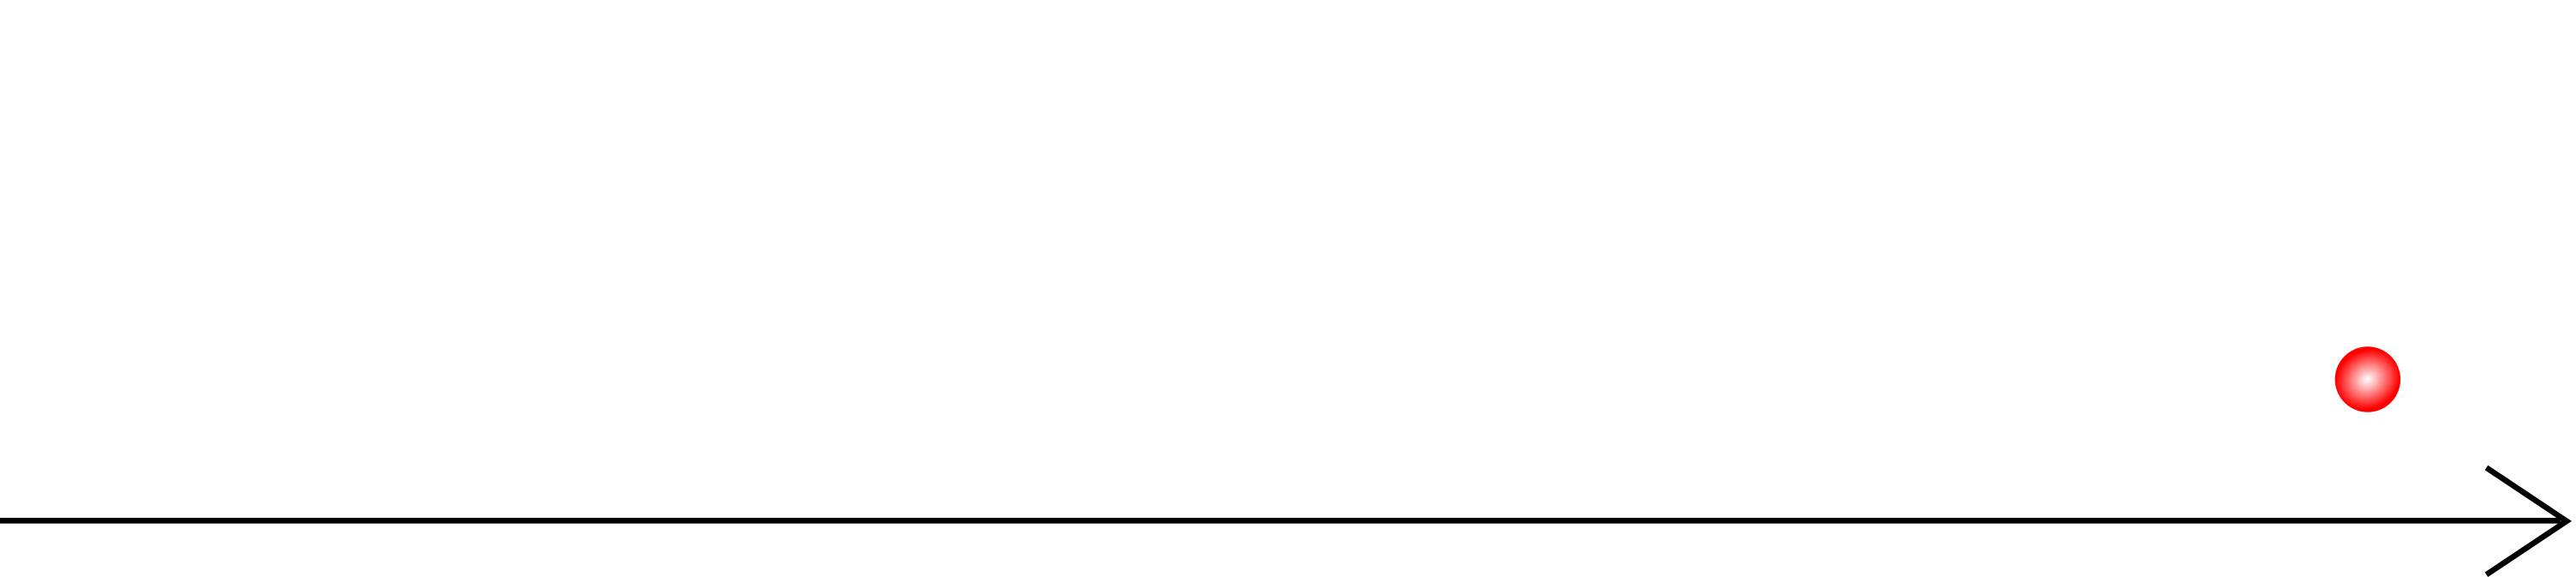
\includegraphics[width=8cm,height=2cm,keepaspectratio]{5beadsMonatomicVsT1.png}
                        \caption{Increasing temperature from left to right.}
                        }
                        \only<2>{
                        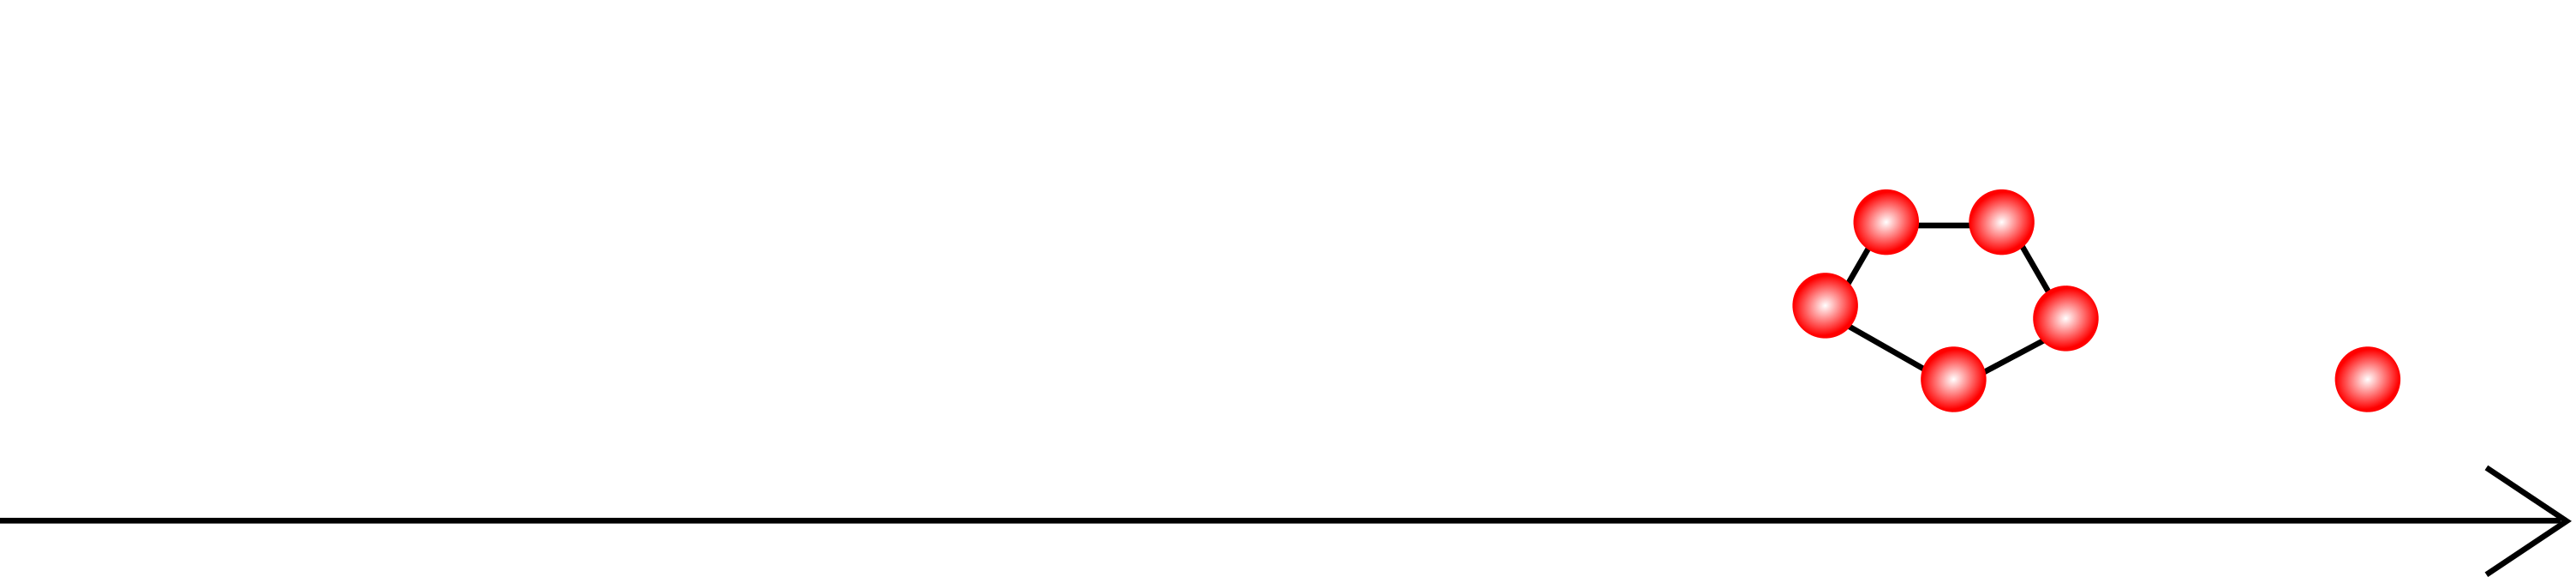
\includegraphics[width=8cm,height=2cm,keepaspectratio]{5beadsMonatomicVsT2.png}
                        \caption{Increasing temperature from left to right.}
                        }
                        \only<3>{
                        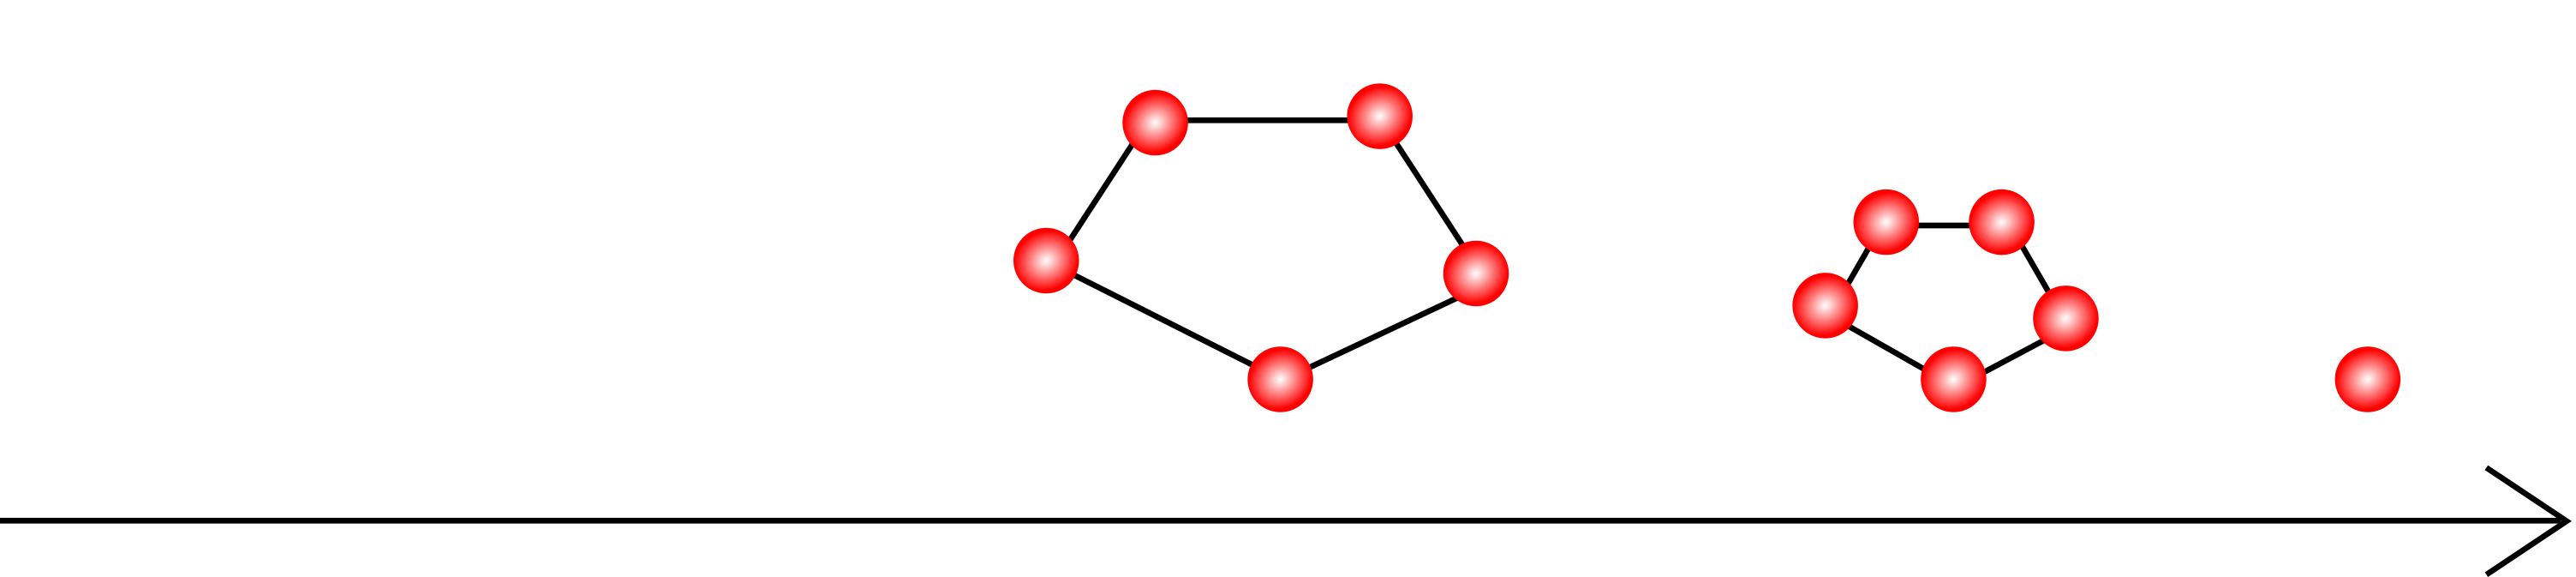
\includegraphics[width=8cm,height=2cm,keepaspectratio]{5beadsMonatomicVsT3.png}
                        \caption{Increasing temperature from left to right.}
                        }
                        \only<4>{
                        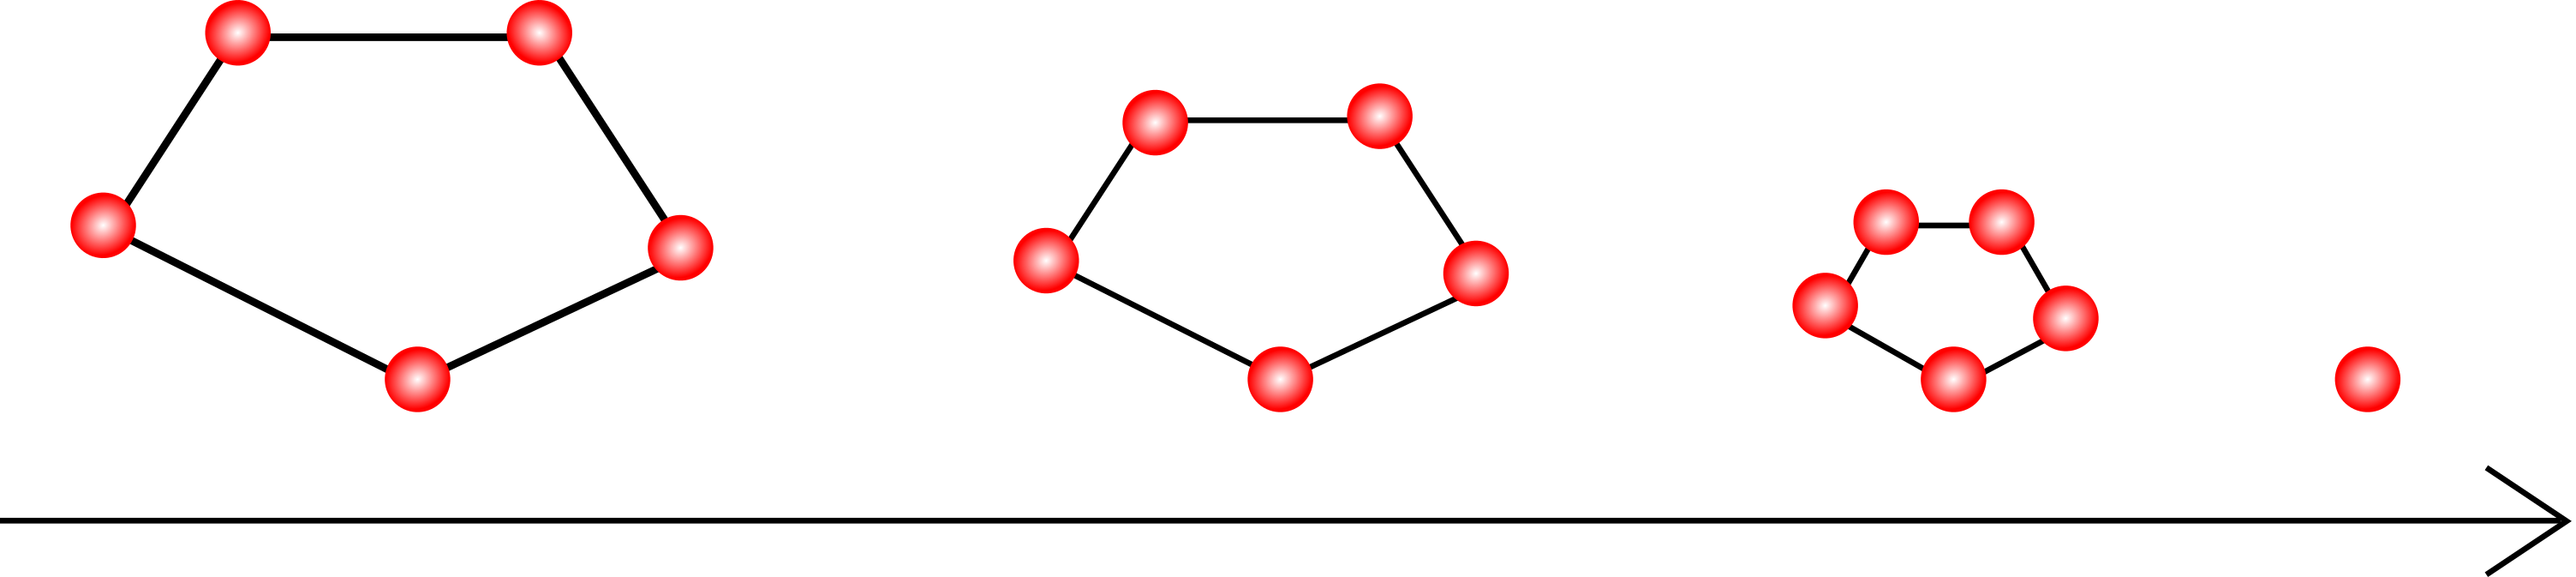
\includegraphics[width=8cm,height=2cm,keepaspectratio]{5beadsMonatomicVsT4.png}
                        \caption{Increasing temperature from left to right.}
                        }
                    \end{figure}
                \end{overlayarea}
            \end{center}
        \end{frame}
        \begin{frame}
            \frametitle{Diatomic molecule - rigid rotor\putCitation{Patkowski2008}}
            \begin{itemize}
                \item Let $m$ and $I$ denote the mass of the atom and moment of inertia of the rigid rotor respectively. Its Hamiltonian is given by:
                    \begin{equation*}
                    \label{eq:hDiatomic}
                        \hat{h}_2 = \displaystyle\frac{\hat{\mbf{p}}^2}{2m} + \frac{\hat{\mbf{J}}_1^2}{2I} + \frac{\hat{\mbf{J}}_2^2}{2I} + \hat{U}(r,\Omega_1,\Omega_2)
                    \end{equation*}
            \end{itemize}
            \begin{block}{Matrix elements}
                \begin{equation*}
                    \begin{aligned}
                        \mc{T}^{i,i+1}_{\text{tra}} = \left< \mbf{x}^i \left| \exp \left(-\displaystyle\frac{\beta \hat{\mbf{p}}^2}{2 m P} \right) \right| \mbf{x}^{i+1} \right> &= \alert<2>{\displaystyle\frac{P^{3/2}}{\Lambda_m^3} \exp \left(-\displaystyle\frac{\pi P (\mbf{x}^i - \mbf{x}^{i+1})^2}{\Lambda_m^2}\right)}\\
                        \mc{T}^{i,i+1}_{\text{rot}} = \left< \Omega^i \left| \exp \left(-\displaystyle\frac{\beta \hat{\mbf{J}}^2}{2IP} \right) \right| \Omega^{i+1} \right> &= \alert<3>{\displaystyle\sum_{j=0}^\infty \frac{2j+1}{4 \pi} \mc{P}_j (cos (\theta_{i,i+1}))}\\
                        &\qquad \alert<3>{\times \exp \left[-\beta j(j+1) \Upsilon/ P \right]}
                    \end{aligned}
                \end{equation*}
            \end{block}
        \end{frame}

        \begin{frame}
            \frametitle{Diatomic molecule - rigid rotor\putCitation{Patkowski2008}}
            \begin{itemize}
                \justifying
                \item Defining $\mbf{r} \equiv \mbf{x}^{(1)}, \mbf{\Delta}^{(i)} \equiv \mbf{x}^{(i+1)} - \mbf{x}^{(i)}$,
                \begin{equation*}
                    \exp [-\beta \bar{U} (|\mbf{r}|)] = \left< \exp \left[ -\frac{\beta}{P} \sum_{i=1}^P U (|\mbf{x}^i|,\Omega_1^i,\Omega_2^i) \right] \right>_{F,\varrho}
                \end{equation*}
                \item Probability distributions:
                \begin{align*}
                    \varrho(\mbf{\Omega}) &= \frac{1}{q_\text{rot}} \displaystyle\prod_{i=1}^P \mc{T}_\text{rot}^{i,i+1}, \qquad F(\mbf{\Delta}) = \Lambda_m^3 \displaystyle\prod_{i=1}^P \mc{T}_\text{tra}^{i,i+1}\\
                    q_{rot} &= \displaystyle\sum_{j'} (2j' + 1) \exp \left[-\beta \Upsilon j' (j'+1) \right]
                \end{align*}
            \end{itemize}
            \begin{block}{Fully quantum second virial coefficient}
                \begin{equation*}
                    \alert{B_2 (T) = -2 \pi \displaystyle\int dr~ r^2 (e^{-\beta \bar{U} (r)} - 1)}
                \end{equation*}
            \end{block}
        \end{frame}
        \begin{frame}
            \frametitle{Diatomic molecule - rigid rotor\putCitation{Patkowski2008}}
            \begin{itemize}
                \justifying
                \item A closer look at the effective potential:
                \begin{equation*}
                    \exp [-\beta \bar{U} (|\mbf{r}|)] = \left< \exp \left[ -\frac{\beta}{P} \sum_{i=1}^P U (|\mbf{x}^i|,\Omega_1^i,\Omega_2^i) \right] \right>_{F,\varrho}
                \end{equation*}
            \end{itemize}
            \begin{figure}
                \centering
                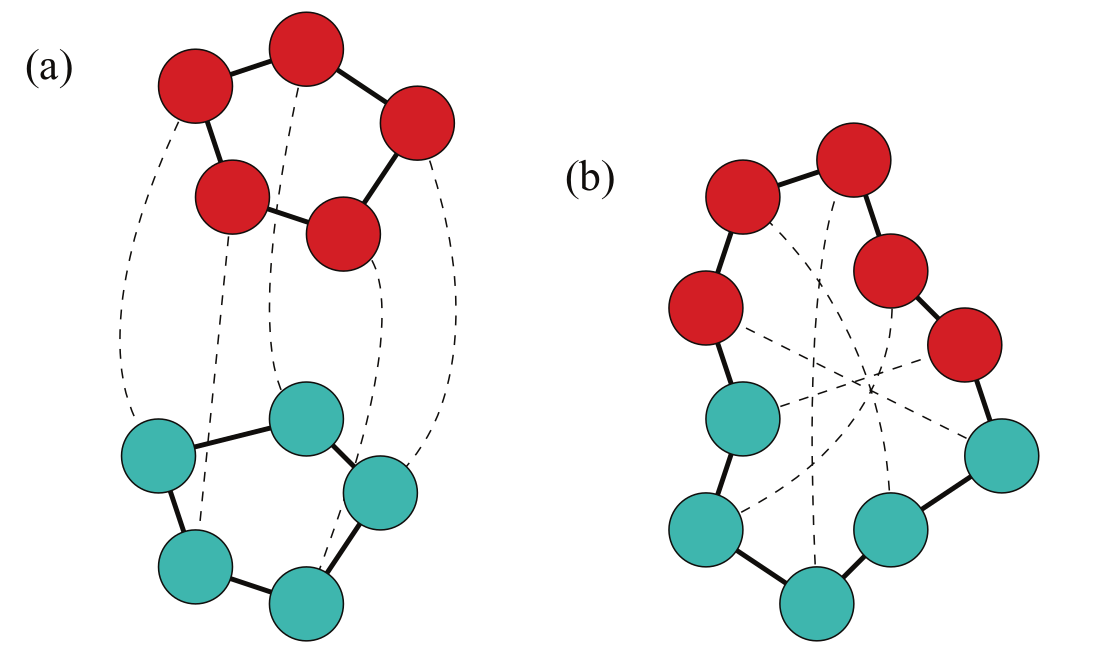
\includegraphics[scale=0.25,keepaspectratio]{BoltzmannXC.png}
                \caption{Boltzmann- and exchange-type conformations shown on the left and right respectively.}
            \end{figure}
        \end{frame}
        \begin{frame}
            \frametitle{Objectives}
            \begin{block}{Diatomic molecules}
                Compute accurate virial coefficients using state-of-the-art \abinitio{} potentials, MSMC and PIMC methods for the rigid case.
            \end{block}
            \begin{alertblock}{Challenges}
                Lack of efficient an sampling algorithm for orientations.
            \end{alertblock}
        \end{frame}

        \subsection{Novel algorithms}
        \begin{frame}
            \frametitle{Orientation sampling}
            \begin{itemize}
                \item Idea proposed by Garberoglio et al. \putCitation{Garberoglio2014}: two independent atoms (vs. one rigid rotor previously).
                \item Leads to possibility of avoiding quantum mechanical calculations.
                \item Sampling problem can be reduced to choosing a ring of beads on the surface of a sphere.
                \item A more viable path to study multiatomic systems.
            \end{itemize}
        \end{frame}
        \iffalse
        \begin{frame}
            \frametitle{Orientation sampling}
            \begin{itemize}
                \item Instead of using Cartesian coordinates, we use the $P$ COM position vectors $\mbf{R}_i$ and the $P$ bead (or image) vectors $\mbf{b}_i$.
                \item We consider both Boltzmann type as well as exchange type configurations.
                \item Probability associated with a configuration $\mbf{Z} \equiv (\mbf{R},\mbf{b})$ is given as:
                \begin{equation*}
                \label{eq:PIProb}
                    P_\sigma (\mbf{Z}) = \frac{1}{Q_1^{{\rm (\sigma)}}} F(\mbf{R};2m) F(\mbf{b}^{(\sigma)};m/2) e^{ - \beta \bar u(\mbf{b})}
                \end{equation*}
                where $F$ is the path-integral weight, and $\bar u$ is the intramolecular potential energy averaged over all images:
                \begin{equation*}
                    \begin{aligned}
                        F(\mbf{x};m) &= \left( \frac{P^{3/2}} {\Lambda _m^3} \right)^P \exp \left[ - \frac{\pi P}{\Lambda _m^2}\sum\limits_{i = 0}^{P-1} \left| \mbf{x}_{i + 1} - \mbf{x}_i \right|^2 \right]\\
                        &\bar u(\mbf{b}) = \frac{1}{P}\sum\limits_{i=0}^{P-1} {u\left(b_i \right)}
                    \end{aligned}
                \end{equation*}
            \end{itemize}
        \end{frame}
        \fi
        \begin{frame}
            \frametitle{Orientation sampling}
            \begin{itemize}
                \item Probability associated with a configuration $\mbf{Z} \equiv (\mbf{R},\mbf{b})$ is given as:
                \begin{equation*}
                \label{eq:PIProb}
                    P_\sigma (\mbf{Z}) = \frac{1}{Q_1^{{\rm (\sigma)}}} F(\mbf{R};2m) F(\mbf{b}^{(\sigma)};m/2) e^{ - \beta \bar u(\mbf{b})}
                \end{equation*}
                \item Define $\pi$ to be the $\mbf{b}$-dependent terms of the path integral weight $F$.
                \item We generate a trial configuration with probability $\tau (o \to n)$, based on an approximation for $\pi$ denoted as $\tilde \pi$, and accept or reject based on:
                \begin{equation*}
                    \label{eq:Pacc}
                    P_{\rm acc} = \text{Min} \left[1, \frac{\pi(n)/\pi(o)}{\tau (o \to n)/\tau (n \to o)} \right]
                \end{equation*}
                where `$o$' and `$n$' denote the old and new configurations respectively.
                \item We derive a simple and analytic expression for $\tau (o \to n)$
            \end{itemize}
        \end{frame}
        \begin{frame}
            \frametitle{Orientation sampling - bisection algorithm}
            \begin{itemize}
                \begin{columns}[c]
                    \column{6cm}
                    \item The choice of orientation of image 0 is arbitrary
                    \item At every stage, we are given two images $\mbf{b}_i, \mbf{b}_k$ and we choose the orientation of image $j = (i + k)/2$.
                    \item We note that $\tilde \pi$ is exact for the last step of the algorithm.
                    \column{3.4cm}
                    \vspace{0cm}
                    \begin{overlayarea}{3.5cm}{3.5cm}
                        \begin{figure}[H]
                            \only<1>{
                            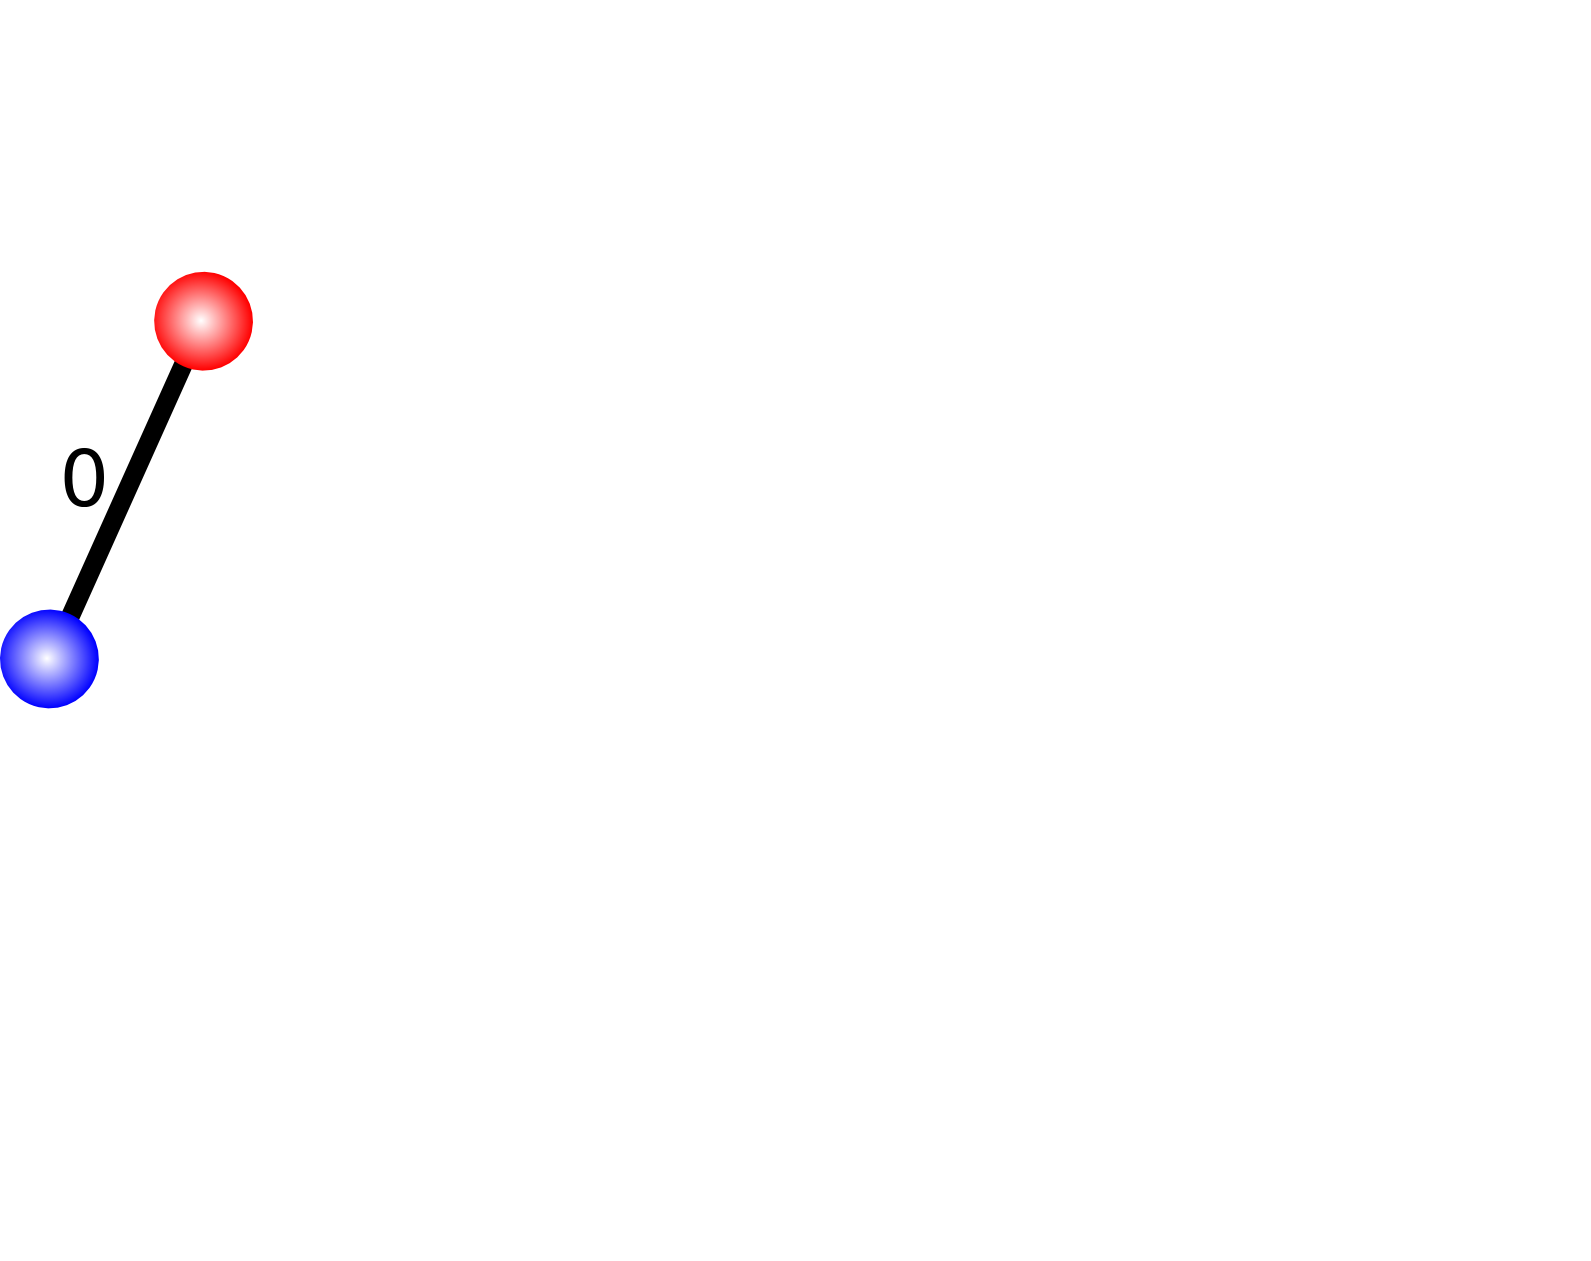
\includegraphics[width=3.5cm,height=3.5cm,keepaspectratio]{ns0.png}
                            \caption{Schematic for P = 8}
                            }
                            \only<2>{
                            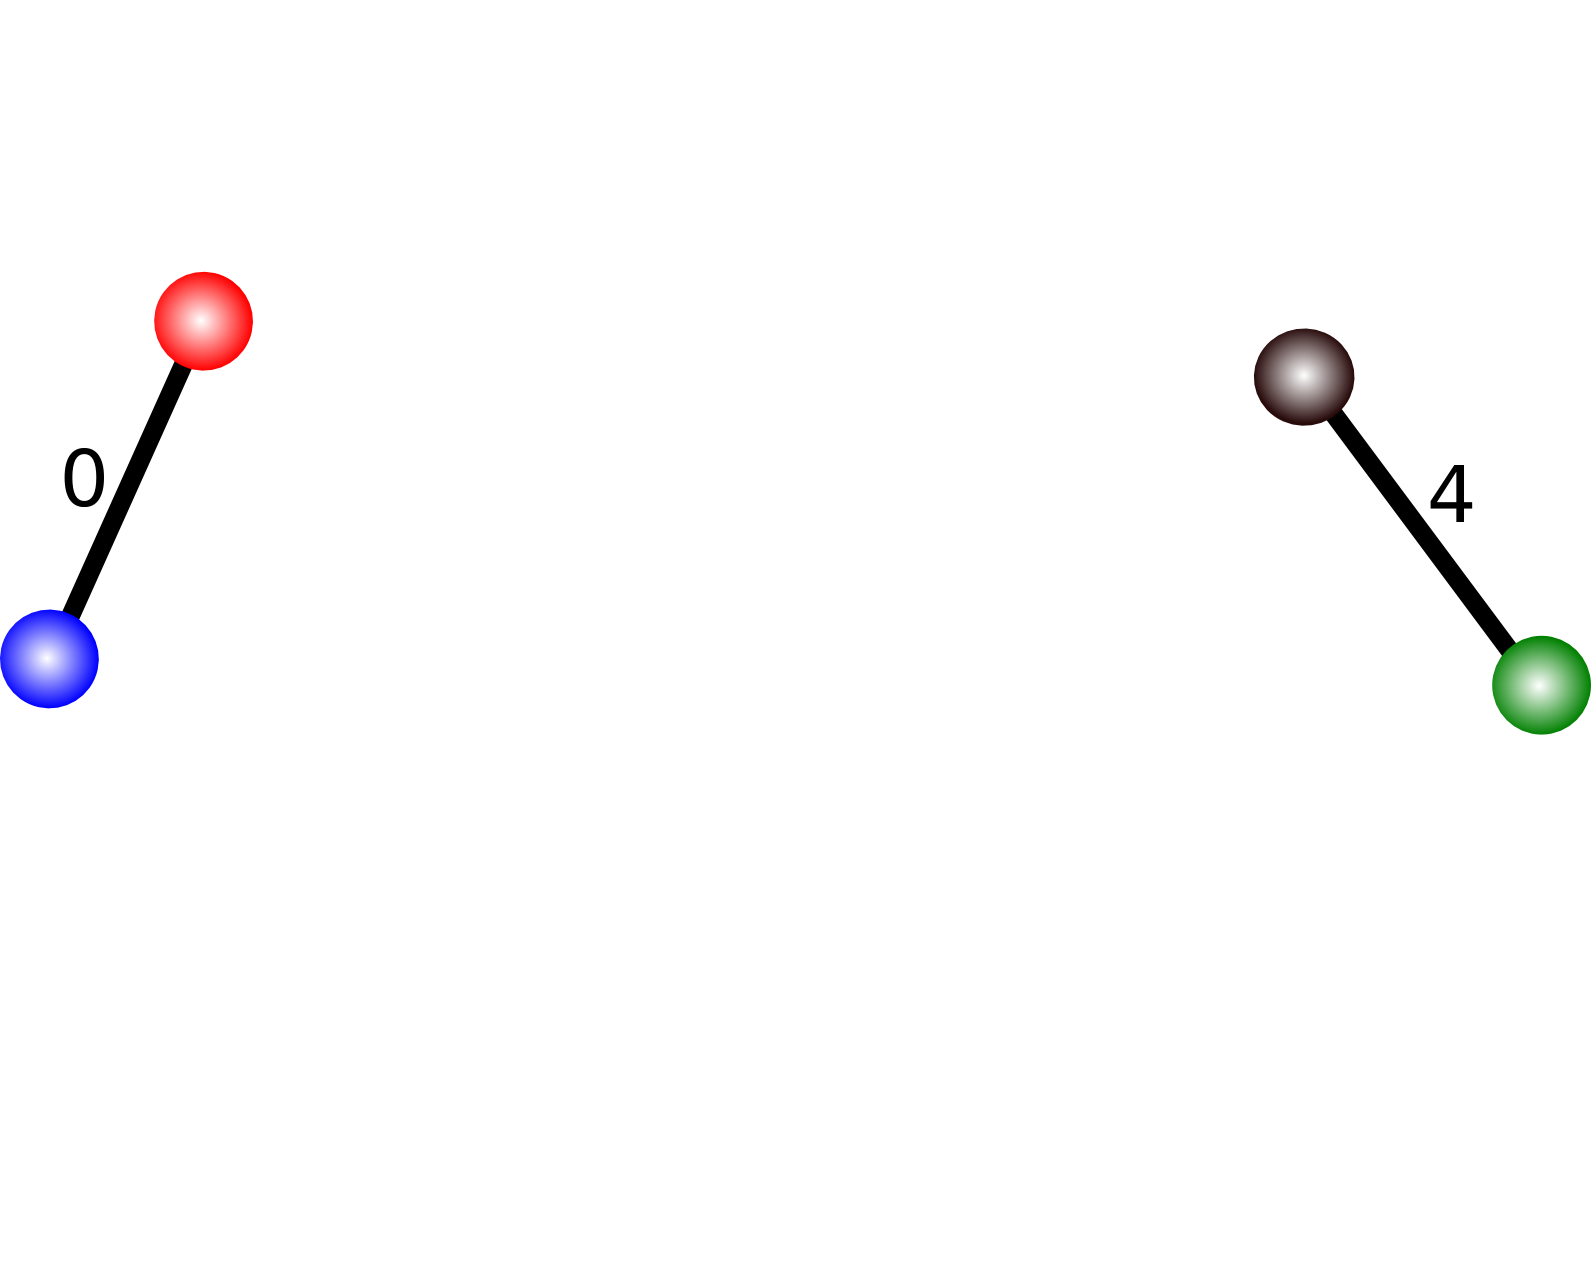
\includegraphics[width=3.5cm,height=3.5cm,keepaspectratio]{ns04.png}
                            \caption{Schematic for P = 8}
                            }
                            \only<3>{
                            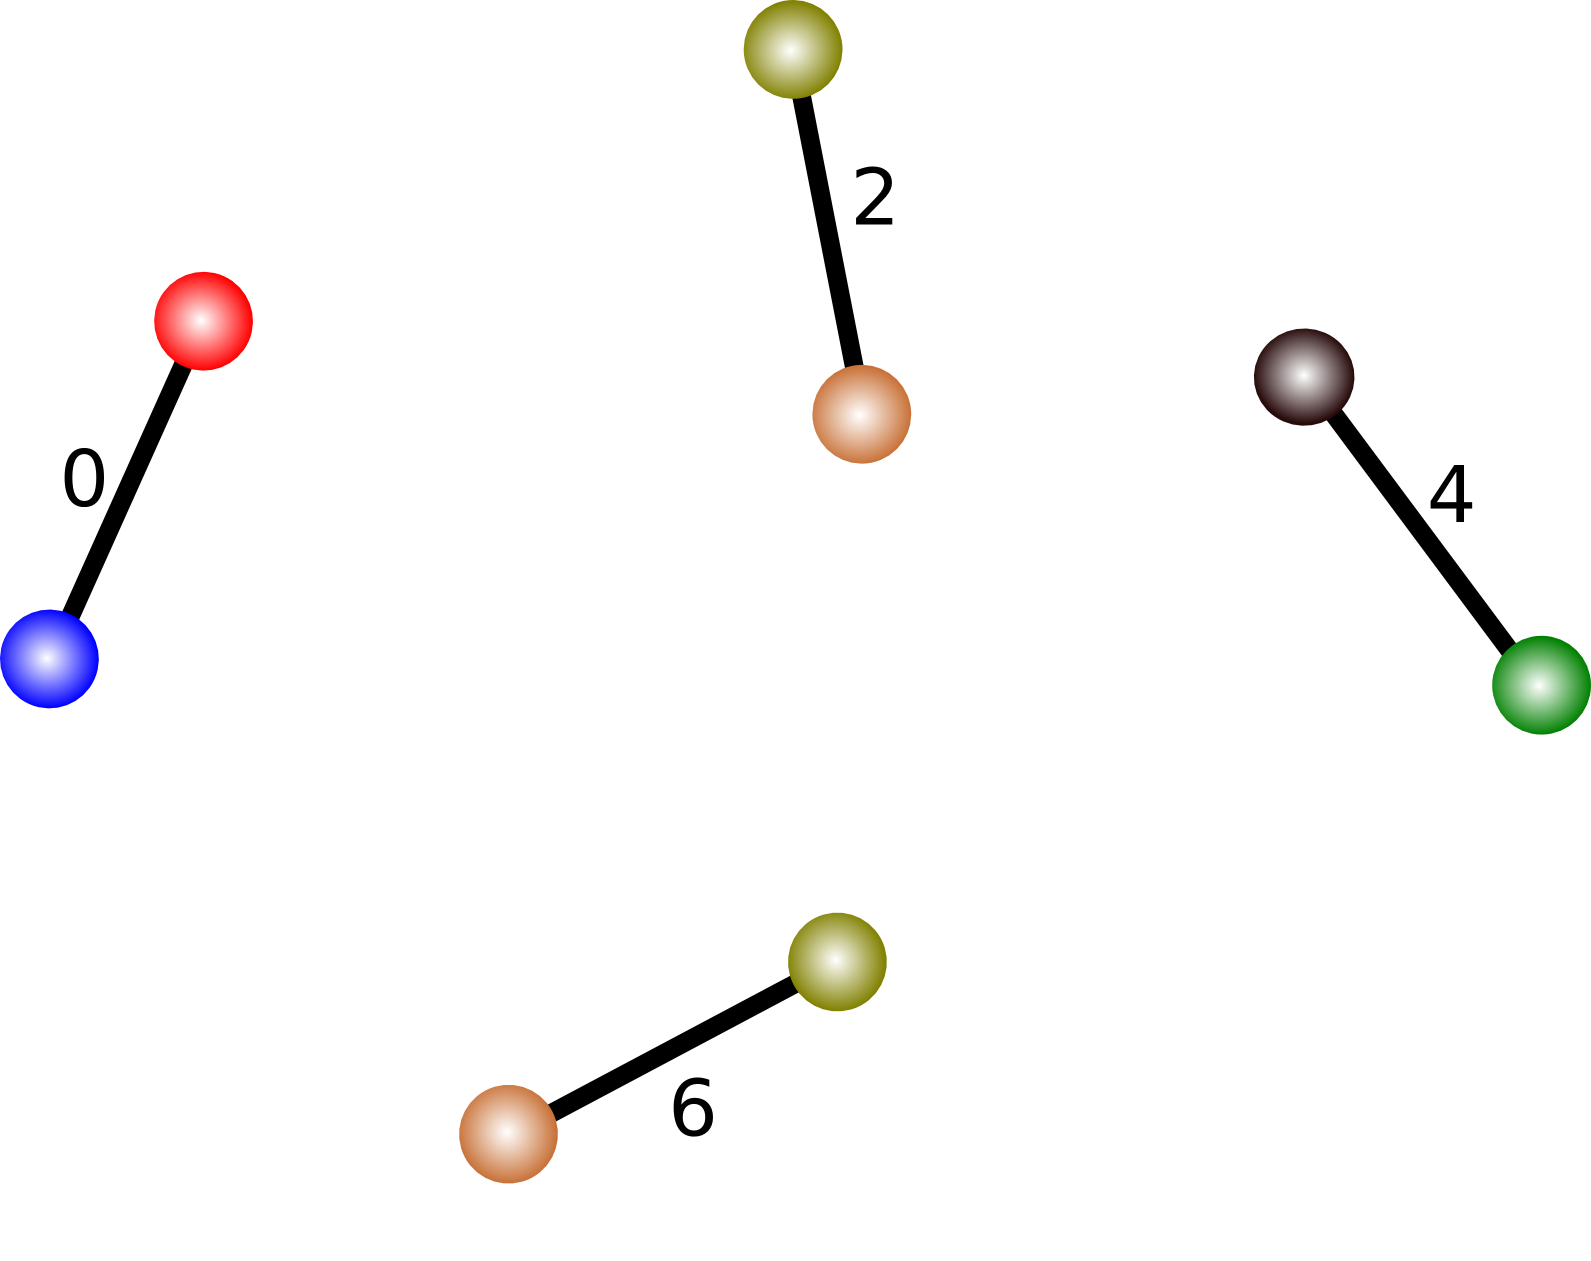
\includegraphics[width=3.5cm,height=3.5cm,keepaspectratio]{ns0426.png}
                            \caption{Schematic for P = 8}
                            }
                            \only<4>{
                            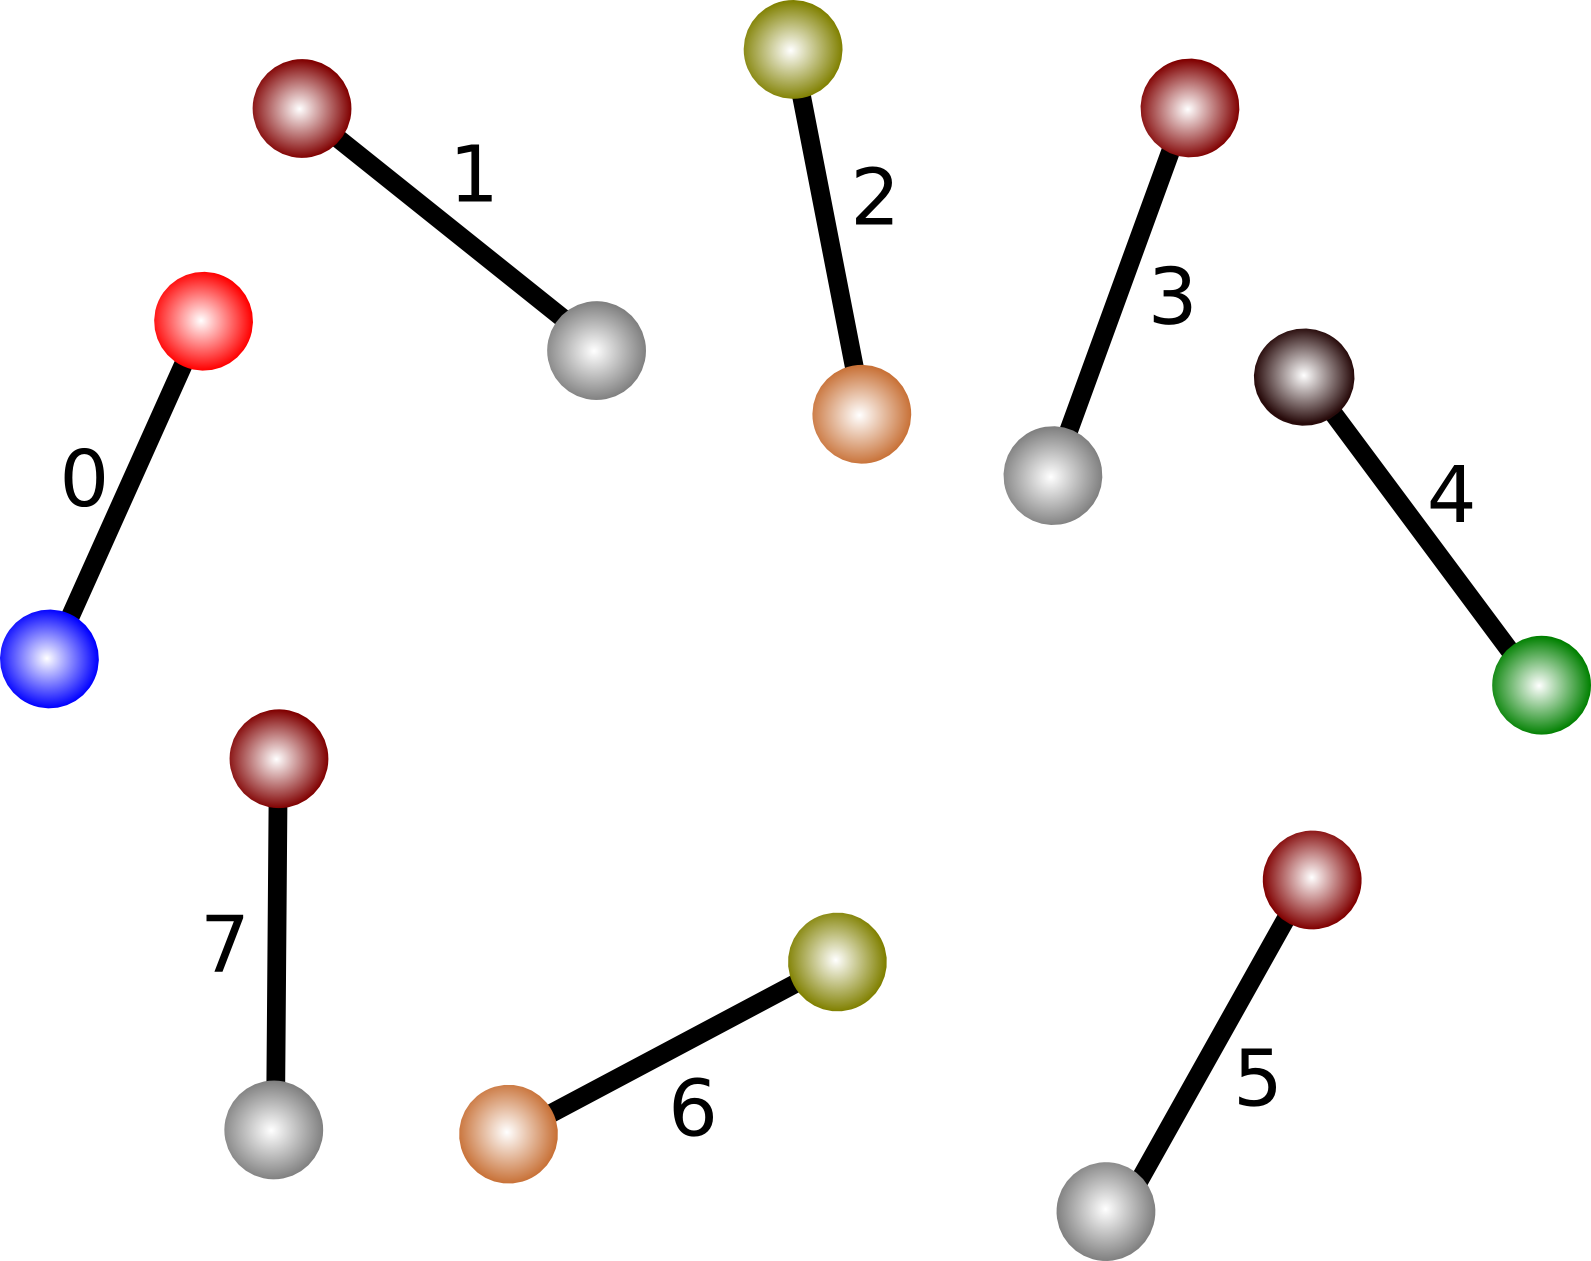
\includegraphics[width=3.5cm,height=3.5cm,keepaspectratio]{nsall.png}
                            \caption{Schematic for P = 8}
                            }
                        \end{figure}
                    \end{overlayarea}
                \end{columns}
            \end{itemize}
        \end{frame}
        \begin{frame}
            \frametitle{Orientation sampling}
            \begin{itemize}
                \begin{columns}[c]
                    \column{6cm}
                    \item Adjacent image probability distribution:
                    \begin{equation*}
                    \label{eq:Uh}
                        \begin{aligned}
                            & \tilde \pi \left( {\mathbf b}_j (\alpha, \beta): \mathbf{a}_j, \psi_{i,k} \right)\\
                            &= \pi({\mathbf b}_i,{\mathbf b}_j)\pi({\mathbf b}_j,{\mathbf b}_k)\\
                            &= \exp\left(-k_h [d_{AC}^2 + d_{BC}^2]\right)\\
                            &= \exp\left(-4 k_h b^2 [1 - \cos(\psi_{i,k}/2) \cos(\alpha)]\right)
                        \end{aligned}
                    \end{equation*}
                    \item The angle $\alpha$ can be calculated by choosing $C$ at random, uniformly on $[0,1]$.
                    \begin{equation*}
                    \label{eq:alpha}
                        \begin{aligned}
                            \alert{\alpha} &= \alert{\cos^{-1} \big[1 +  (1/\kappa)}\\
                            &\alert{\qquad \times \ln\left(1 - C (1-\exp[-2\kappa]) \right) \big]},\\
                            \kappa &= 4 \cos(\psi_{i,k}/2) k_h~b^2
                        \end{aligned}
                    \end{equation*}
                    \column{3.4cm}
                    \begin{figure}[H]
                        \centering
                        \def\svgwidth{\columnwidth}
                        \input{distanceNew1.pdf_tex}
                        \caption{Simplified picture}
                        \label{fig:simple}
                    \end{figure}
                \end{columns}
            \end{itemize}
        \end{frame}

        \begin{frame}
            \frametitle{Objectives}
            \begin{block}{Diatomic molecules}
                Compute accurate virial coefficients using state-of-the-art \abinitio{} potentials, MSMC and PIMC methods for the flexible case.
            \end{block}
                \begin{alertblock}{Challenges}
                    To include vibrational degrees of freedom.
                \end{alertblock}
        \end{frame}
        \begin{frame}
            \frametitle{Methods to handle flexibility}
            \begin{itemize}
                \justifying
                \item Instead of using ground state bond length ($r_0$) use average bond length at each temperature ($< r >_T$)\putCitation{Garberoglio2012}.
                \item Average the entire intermolecular potential ($<U>_T$) over internal degrees of freedom of each monomer, weighted by the appropriate wave function\putCitation{Garberoglio2014}.
                \item Average the intermolecular potential over all four ring polymer configurations and two types of conformations to get an expression for the quantum virial coefficient including monomer flexibility\putCitation{Garberoglio2014}.
            \end{itemize}
        \end{frame}
        \begin{frame}
            \frametitle{Bond-length sampling}
            \begin{itemize}
                \item Define $\pi$ in a similar fashion to the orientation sampling algorithm:
                \begin{equation*}
                    \begin{aligned}
                        \pi(\mathbf{b}) &= \displaystyle\prod\limits_{i=0}^{P-1} b_i^2 e^{-\beta u(b_i)/P} \pi(b_i,b_{i+1},\theta_{i,i+1}) \\
                        \pi(b_i,b_j,\theta_{i,j}) &= \exp\left(-\frac{1}{2}  k_h  \left( b_i^2 + b_j^2 - 2  b_i  b_j  \cos (\theta_{i,j}) \right)\right)\\
                    \end{aligned}
                \end{equation*}
                where $\theta_{i,j}$ is the angle between orientations of images $i$ and $j$.
            \end{itemize}
        \end{frame}
        \begin{frame}
            \frametitle{Bond-length sampling}
            \begin{itemize}
                \item Let $\pi(\mathbf{b}) = $~$ \exp (-y)$, where $y$ can be defined as follows:-
                \begin{equation*}
                \label{eq:y}
                    y = \displaystyle\sum\limits_{i=0}^{P-1} \Bigg\{ k_h  \Big( b_i^2 - b_i  b_j  \cos (\theta_{ij}) \Big) - 2  \log b_i + \frac{ \beta  u (b_i)}{P} \Bigg\}
                \end{equation*}
                \item We define $\tilde y \approx y$ such that:
                \begin{equation*}
                \label{eq:ytilde}
                    \tilde y = \displaystyle\sum\limits_{i=0}^{P-1} \Bigg\{ k_h  \Big( b_i^2 - b_i  b_j \Big) - \frac{2  \log b_i}{P} + \frac{ \beta  u (b_i)}{P} \Bigg\}
                \end{equation*}
                \item We solve for the nominal $\cos (\hat \theta)$ value by:
                \begin{equation*}
                \label{eq:thetaHat}
                    \frac{\partial y}{\partial b_i} = \frac{\partial \tilde y}{\partial b_i} \Rightarrow \cos (\hat \theta) = 1 - \frac{P-1}{P~k_h~b_i^2}
                \end{equation*}
                \item Using this nominal value in the expression for $y$, we find $b_m$ such that:
                \begin{equation*}
                \label{eq:bm}
                    \displaystyle\frac{\partial y}{\partial b_i} \bigg|_{b_i = b_m} = 0 \qquad \forall i
                \end{equation*}
            \end{itemize}
        \end{frame}
	\section{Results}
        \subsection{Hydrogen}
            \begin{frame}
                \frametitle{$B_2$ values for Hydrogen compared with Garberoglio et al.\putCitation{Garberoglio2014}.}
                \begin{center}Bond length: $< r >_0$, total configuration samples: 10$^7$.\end{center}
                \begin{figure}
                    \centering
                    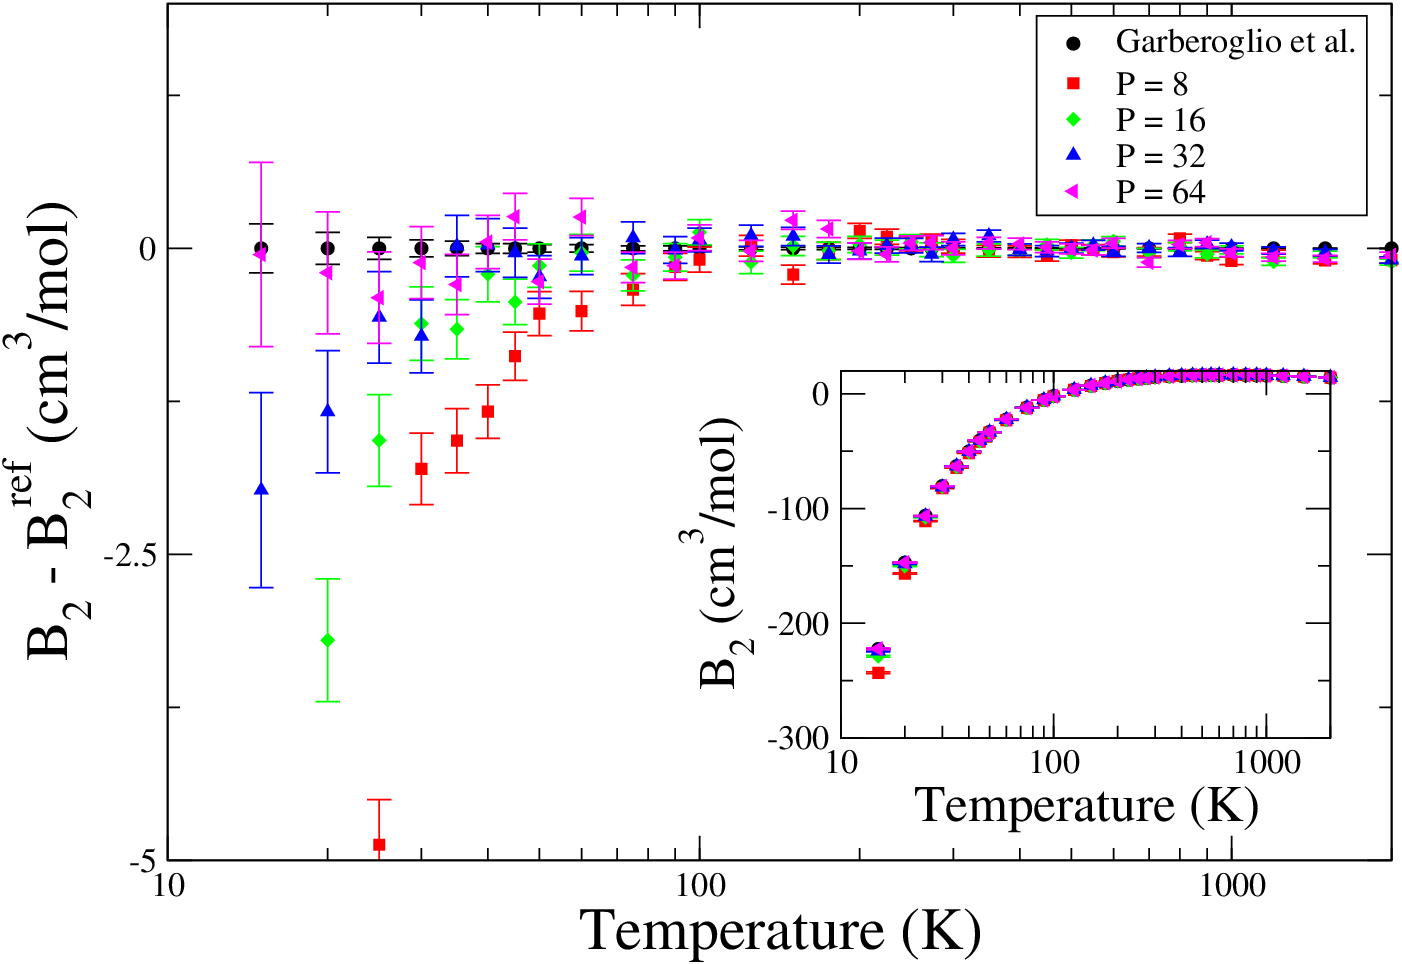
\includegraphics[scale=0.18,keepaspectratio]{s1GarberoglioAll.png}
                \end{figure}
            \end{frame}
            \begin{frame}
                \frametitle{$B_2$ values for Hydrogen compared with Goodwin et al.\putCitation{Goodwin1963}.}
                \begin{center}Bond length: $< r >_0$, total configuration samples: 10$^7$.\end{center}
                \begin{figure}
                    \centering
                    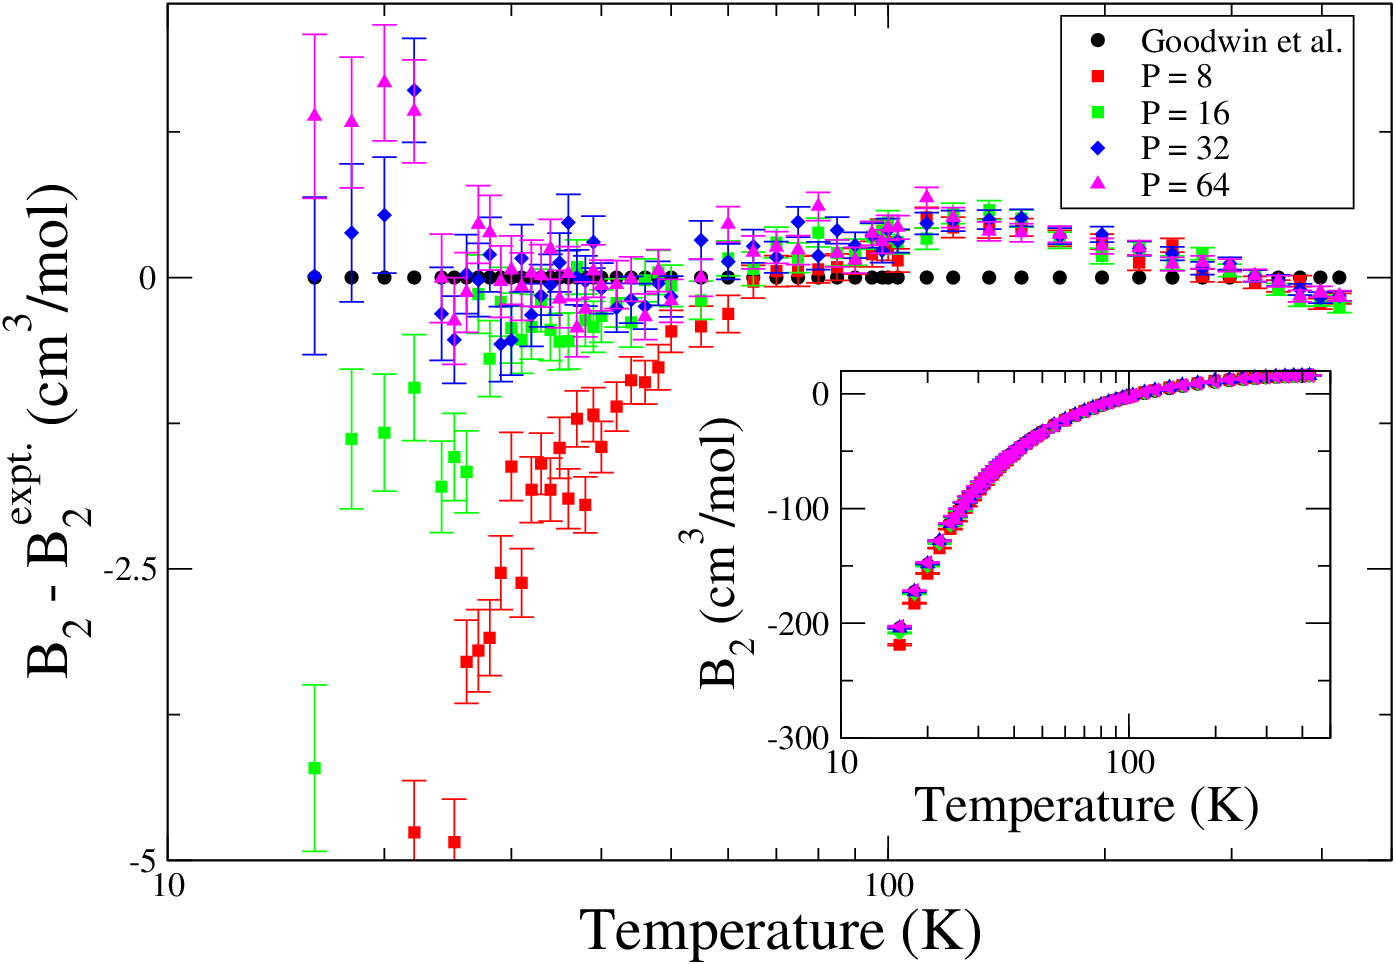
\includegraphics[scale=0.18,keepaspectratio]{s1GoodwinAll.png}
                \end{figure}
            \end{frame}
            \begin{frame}
                \frametitle{$B_2$ values for Hydrogen compared with Garberoglio et al.\putCitation{Garberoglio2014}.}
                \begin{center}Bond length: $< r >_T$, total configuration samples: 10$^7$.\end{center}
                \begin{figure}
                    \centering
                    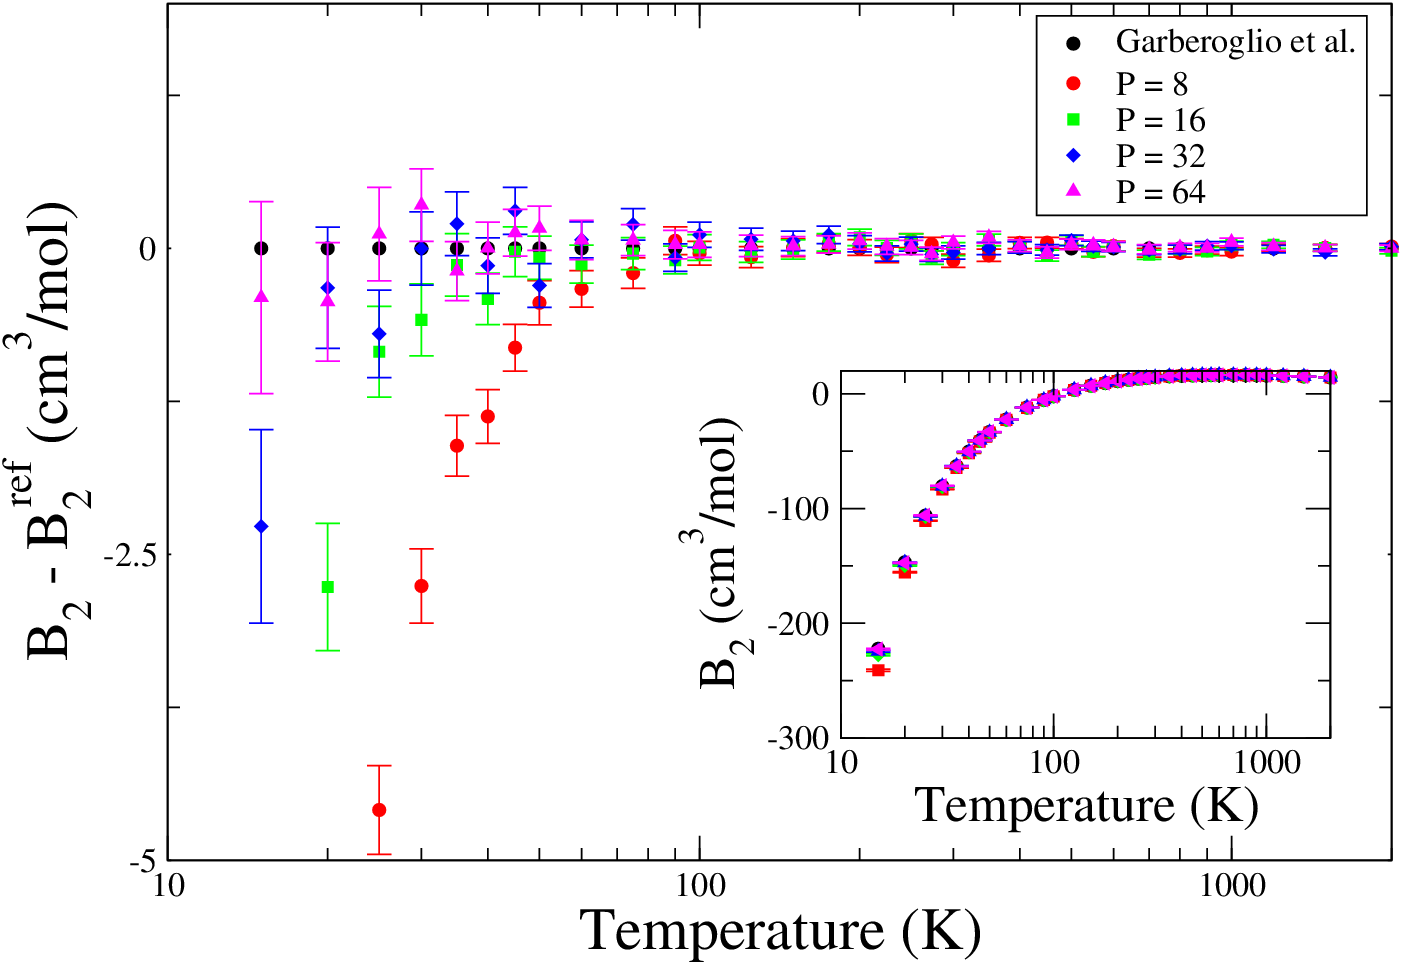
\includegraphics[scale=0.18,keepaspectratio]{s2GarberoglioAll.png}
                \end{figure}
            \end{frame}
            \begin{frame}
                \frametitle{Performance of the orientation move.}
                \begin{figure}
                    \centering
                    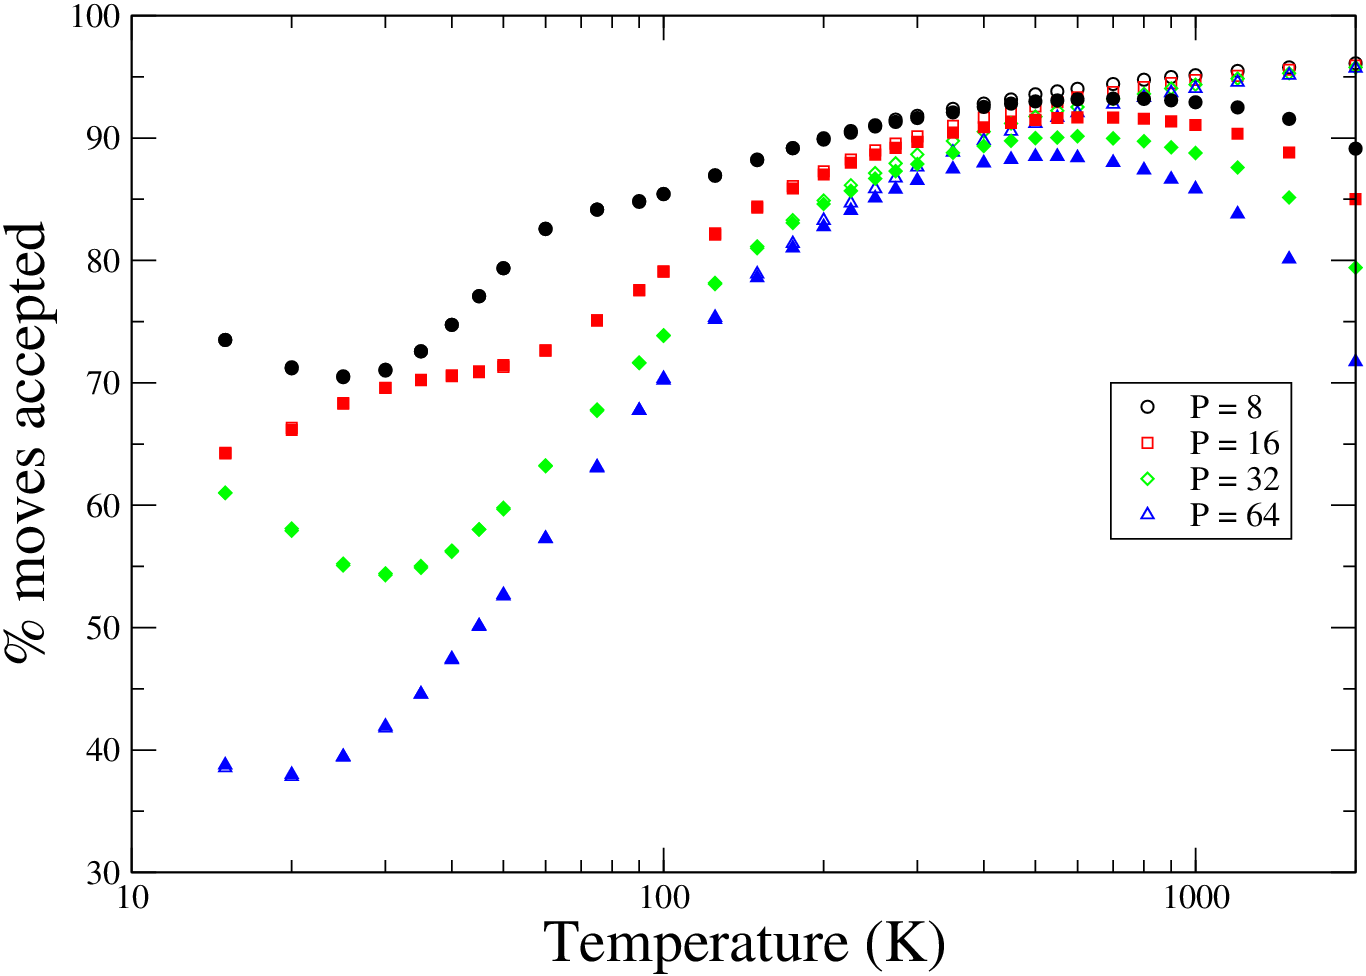
\includegraphics[scale=0.18,keepaspectratio]{s12orAcc.png}
                \end{figure}
            \end{frame}
            \begin{frame}
                \frametitle{$B_2$ values for Hydrogen compared with Garberoglio et al.\putCitation{Garberoglio2014}.}
                \begin{center}Bond length: variable, total configuration samples: 10$^7$.\end{center}
                \begin{figure}
                    \centering
                    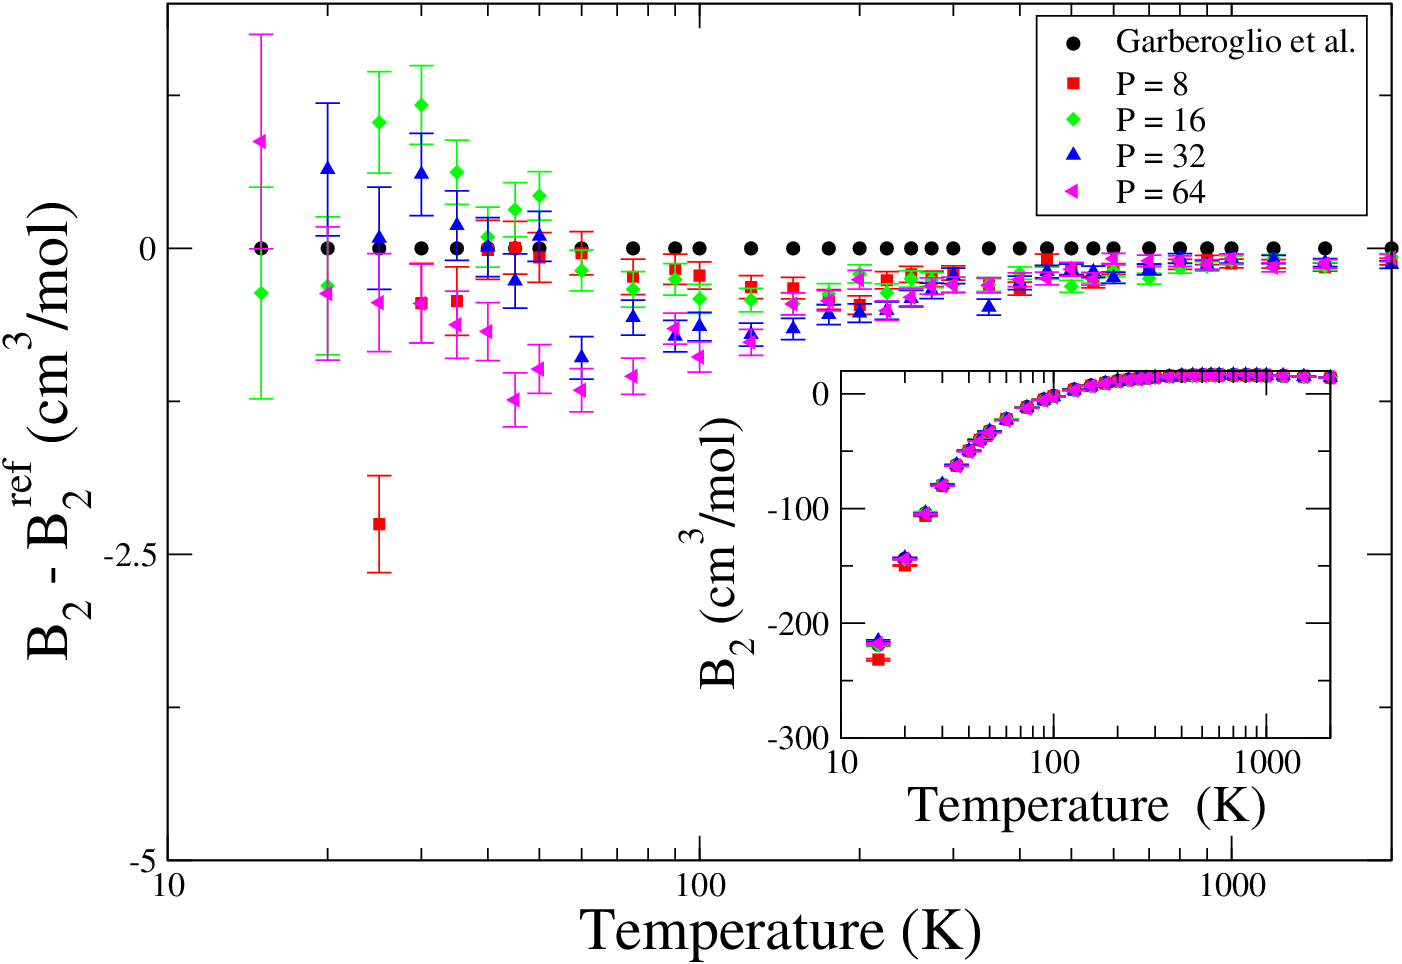
\includegraphics[scale=0.18,keepaspectratio]{s3GarberoglioAll.png}
                \end{figure}
            \end{frame}
        \subsection{Nitrogen}
            \begin{frame}
                \frametitle{$B_2$ values for Nitrogen compared with Hellmann\putCitation{Hellmann2013}.}
                \begin{center}Total configuration samples: 10$^9$ for cl, sc and 10$^8$ for all PI cases.\end{center}
                \begin{figure}[!htbp]
                    \centering
                    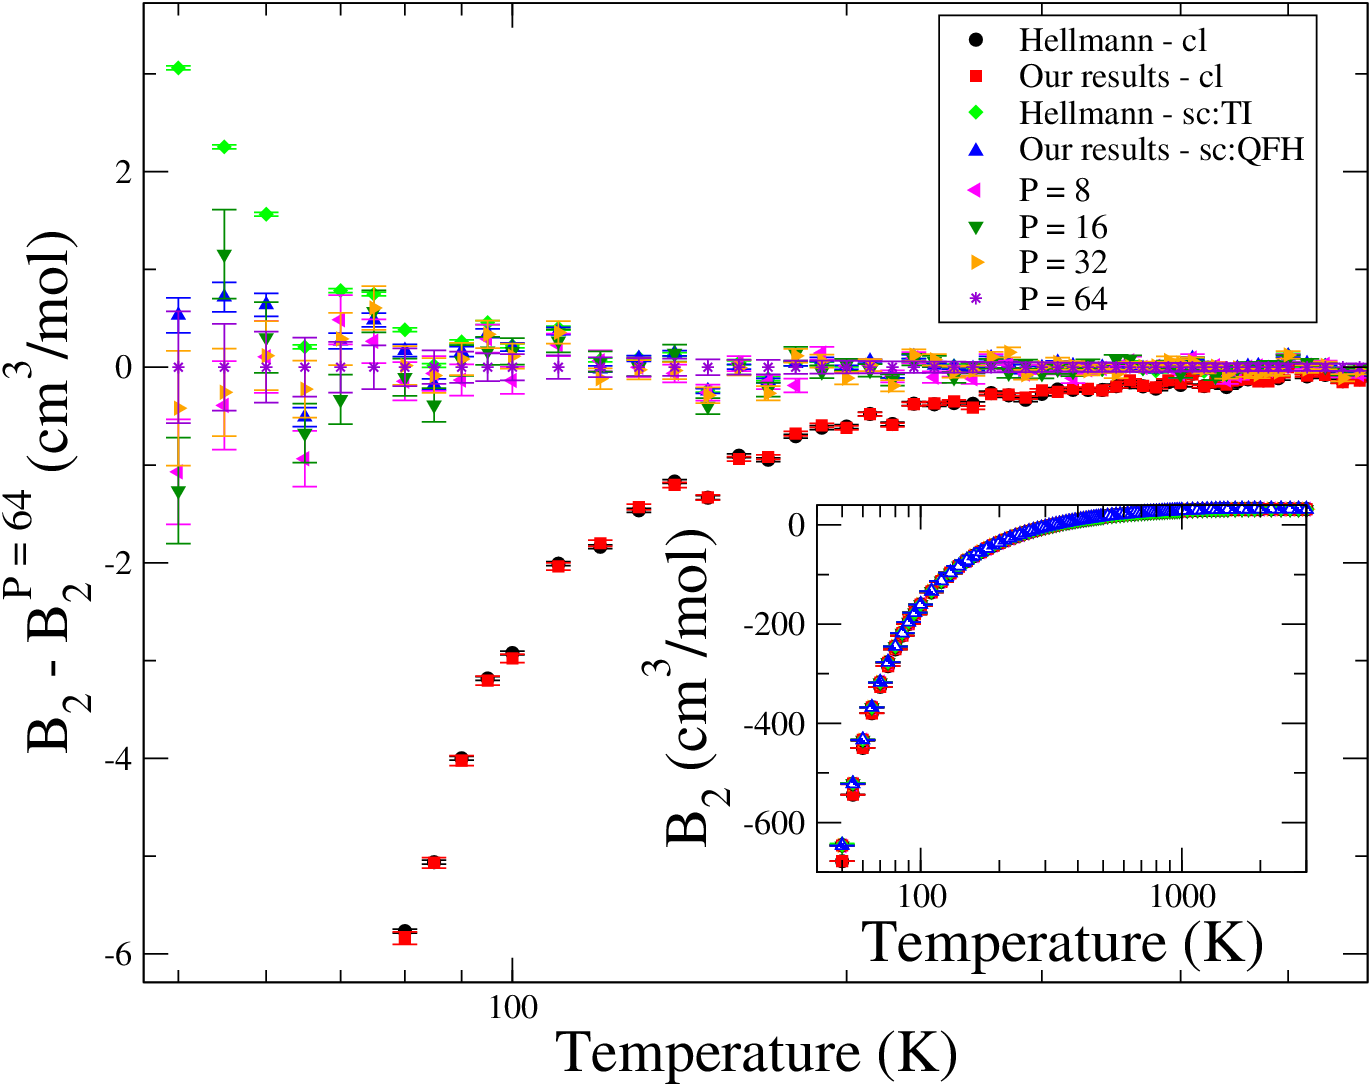
\includegraphics[scale=0.15,keepaspectratio]{B2AllDiffPICB.png}
                \end{figure}
            \end{frame}
        \subsection{Oxygen}
            \begin{frame}
                \frametitle{$B_2$ values for Oxygen compared with Bartolomei et al.\putCitation{Bartolomei2010}.}
                \begin{center}PES: PT2, Total configuration samples: 10$^8$ for cl and 10$^7$ for all PI cases. Experimental\putCitation{Dymond}, SC - Perugia \putCitation{Aquilanti1999,Bartolomei2010}.\end{center}
                \begin{figure}[!htbp]
                    \centering
                    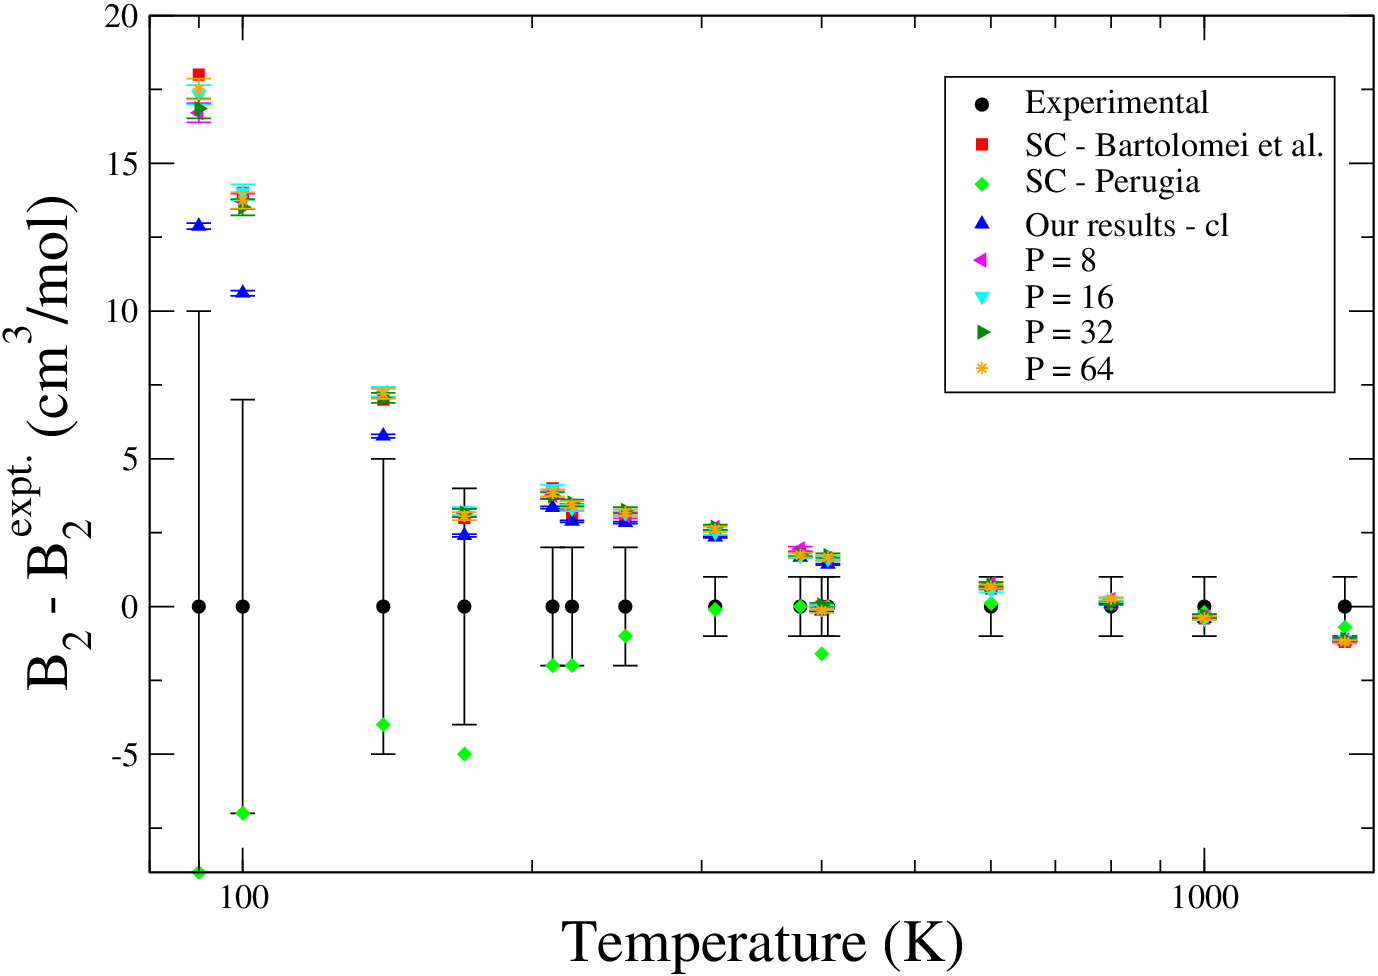
\includegraphics[scale=0.12,keepaspectratio]{B2O2AllExpDiffPT2.png}
                \end{figure}
            \end{frame}

	\section{Summary}
        \begin{frame}
            \frametitle{Conclusion}
            \begin{figure}[!htbp]
                \centering
                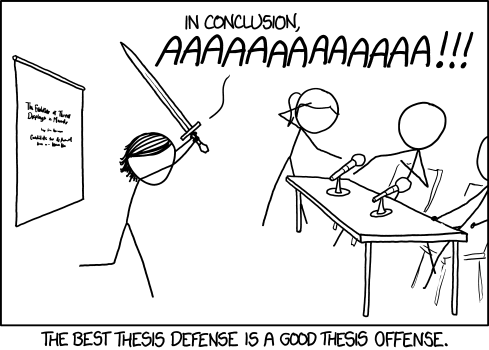
\includegraphics[scale=0.6,keepaspectratio]{thesis_defense.png}
                \caption{\tiny{https://xkcd.com/1403/}}
            \end{figure}
        \end{frame}
        \begin{frame}
            \frametitle{Summary}
            \begin{itemize}
                \item We have developed two direct sampling algorithms for orientations and bond-lengths of diatomic molecules.
                \item Fundamental to both these algorithms is the idea of treating the two atoms independently as opposed to a rigid rotor.
                \item Owing to the simple nature of the probability distributions, our algorithms are efficient.
                \item We have tested these algorithms by computing quantum virial coefficients using PIMC method for three different diatomic systems.
                \item We observed overall good agreement with literature values for the temperatures considered.
                \item For nitrogen and oxygen, lower temperatures need to be considered for quantum effects to be significant. 
            \end{itemize}
        \end{frame}
        \begin{frame}
            \frametitle{Future direction of work}
            \begin{block}{Analysis}
                \begin{itemize}
                    \item More detailed analysis to identify sources of inefficiency.
                    \item A rigorous comparison of computational performance with existing algorithms could provide useful insight, or at the very least, lead to quantification of the effort saved.
                \end{itemize}
            \end{block}
            \begin{block}{Application}
                \begin{itemize}
                    \item Isotopes of hydrogen - D$_2$, T$_2$, HD and HT.
                    \item Mixtures of diatomic molecules - O$_2$ + N$_2$, O$_2$ + H$_2$.
                \end{itemize}
            \end{block}
            \begin{block}{Development}
                \begin{itemize}
                    \item Extension of these algorithms to multiatomic systems. Linear multiatomics ,e.g., CO$_2$ could be a first step.
                \end{itemize}
            \end{block}
        \end{frame}

	\section*{Acknowledgments}
    \section*{Appendix}
    \iffalse
        \begin{frame}
            \frametitle{Computational details}
            \begin{itemize}
                \item A short equilibration simulation is performed at the beginning to determine $\alpha$ and to adjust MC move step sizes so that the acceptance of all the MC moves is 50\%.
                \item Irrespective of their number, all MC moves are chosen with equal probability for both the systems within the simulation.
                \item The total number of configuration samples is divided into blocks of 1000 samples each. We compute averages across all blocks for the four ratios and use standard error propagation formulas to arrive at the final result.
                \item Error bars shown represent one standard deviation of the mean (68\% confidence interval).
            \end{itemize}
        \end{frame}

	\begin{frame}
	\frametitle{Bond length\putCitation{Garberoglio2014} - $< r >_T$}
	\begin{figure}
	\centering
	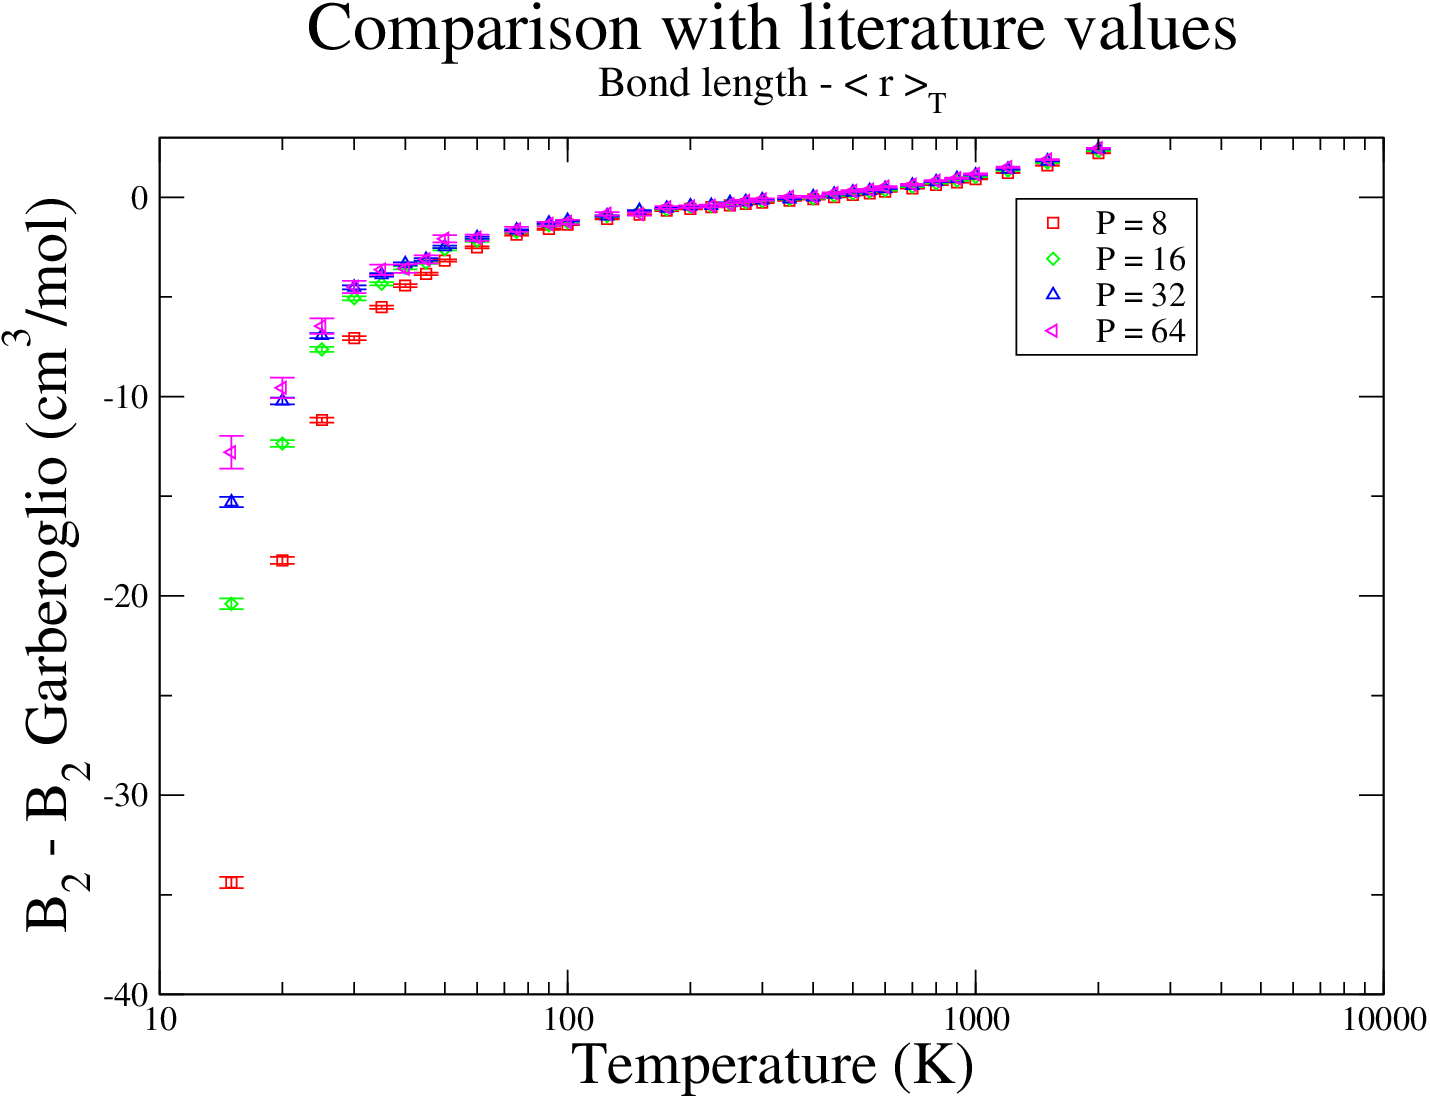
\includegraphics[scale=0.18,keepaspectratio]{8sfTAResultsDiff.png}
	\end{figure}
	
	\end{frame}
    \iffalse
	\begin{frame}
	\frametitle{Bond length sampling - Introduction}
	\begin{itemize}
	\justifying
	\item Harmonic energy ($U_h$) of the springs and the intra-molecular potential energy ($U_i$) are the only two factors that affect the probability $\mathcal{P}$ of an image
	\item $U_h$ for adjacent monomers is given by:
	\begin{figure}
	\centering
	\def\svgscale{0.2}
	\input{uHarmonic.pdf_tex}
	\end{figure}
	\begin{equation*}
	\begin{aligned}
	U_h &= \frac{1}{2} \cdot k_h \cdot \displaystyle\sum\limits_{i=0}^P \Big( b_i^2 + b_j^2 - 2 \cdot b_i \cdot b_j \cdot \cos (\theta_{ij}) \Big)\\
	\text{where,} \: j &= i - 1 \: \text{for} \: i \ge 1 , j = P - 1\: \text{for} \: i = 0
	\end{aligned}
	\end{equation*}
	\item Intra-molecular potential that we use in our calculations is from Mielke et al.\putCitation{Mielke2002}
	\end{itemize}
	\end{frame}
    \fi
	\begin{frame}
	\frametitle{$\mathcal{P}$ - actual probability of a configuration}
	\begin{itemize}
	\justifying
	\item Expression for $\mathcal{P}$ is almost exponential
	\item Consider the argument of the exponential
	\begin{equation*}
	- \log \mathcal{P} = \displaystyle\sum\limits_{i=0}^P \Bigg\{ k_h \cdot \Big( b_i^2 - b_i \cdot b_j \cdot \cos (\theta_{ij}) \Big) - 2 \cdot \log b_i + \frac{ \beta \cdot U_i (b_i)}{P} \Bigg\}
	\end{equation*}
	\item We can clearly see that it is not quadratic due to the presence of $U_i$
	\item Presence of cross terms such as $b_i \cdot b_j$ makes the bond lengths non-independent of each other
	\end{itemize}
	\end{frame}
	
    \iffalse
	\begin{frame}
	\frametitle{Normal mode analysis}
	\begin{columns}[c]
	\begin{column}{6cm}
	\begin{itemize}
	\justifying
	\item Helps choose all bond lengths simultaneously
	\item Consider the combined behavior of all bond lengths as separate modes
	\item Construct matrix with second derivatives of $- \log \mathcal{P}$
	\item Compute eigenvalues $\lambda_i$ and eigenvectors $\vec{A_i}$ to separate out independent modes
	\item Evaluate new bond lengths simultaneously
	\end{itemize}
	\end{column}
	\begin{column}{4cm}
	\begin{figure}
	\centering
	\def\svgscale{0.3}
	\input{differentModes.pdf_tex}
	\end{figure}
	\end{column}
	\end{columns}
	\end{frame}
    \fi

	\begin{frame}
	\frametitle{Bond length\putCitation{Garberoglio2014} - flexible}
	\begin{figure}
	\centering
	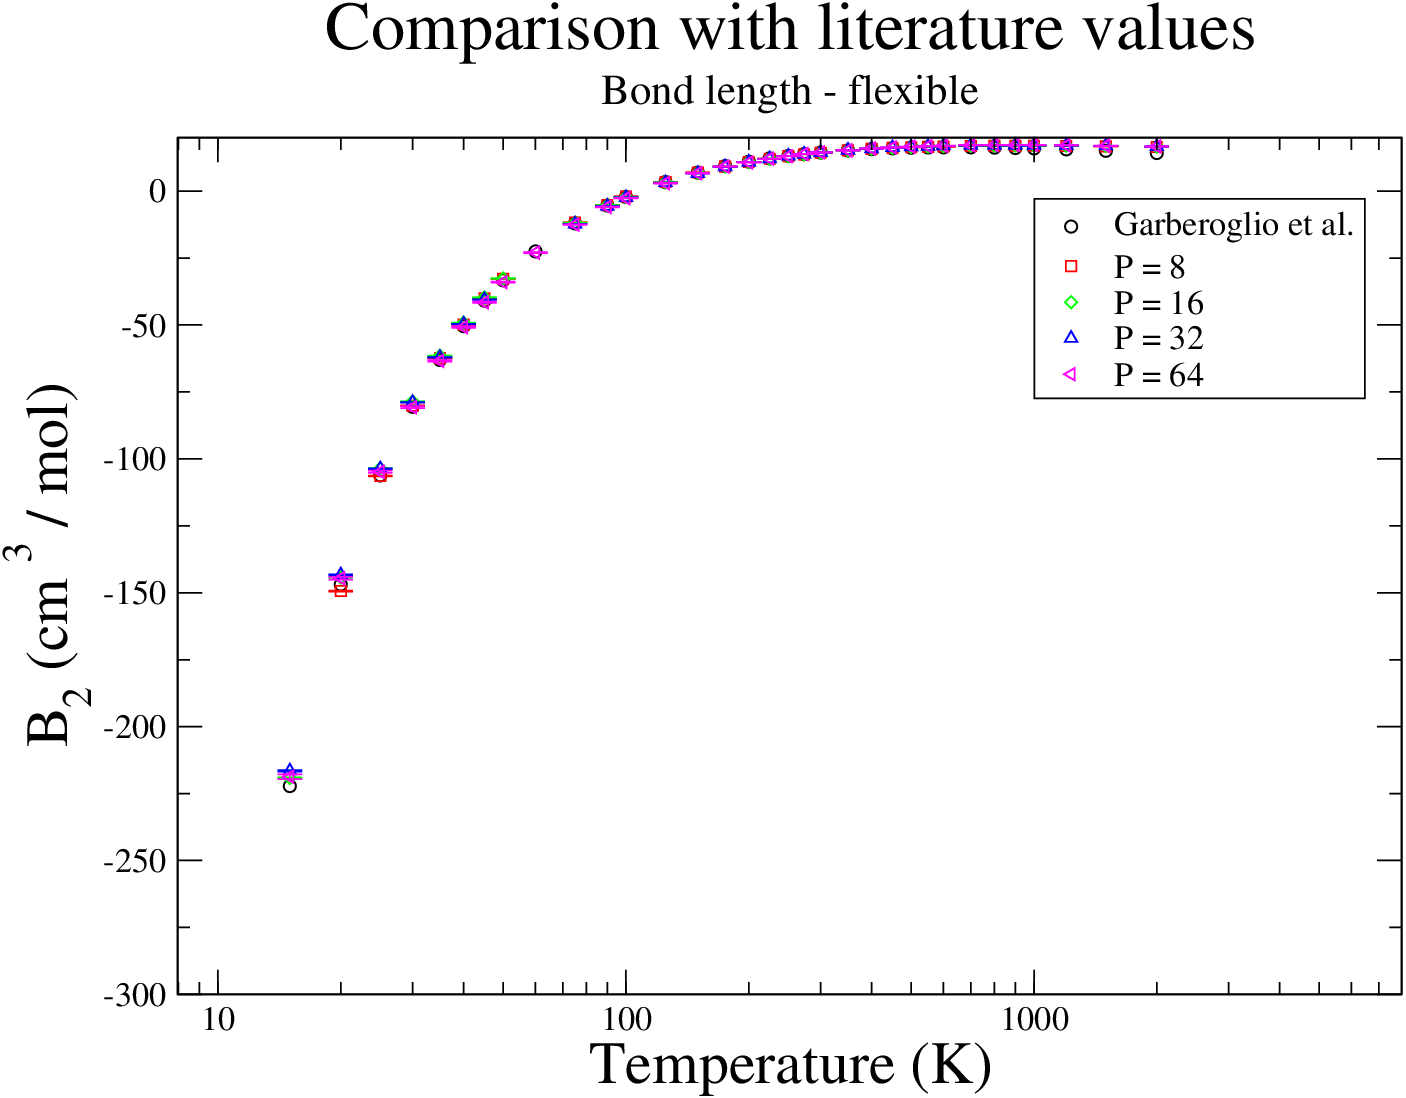
\includegraphics[scale=0.18,keepaspectratio]{8svBLResults.png}
	\end{figure}
	
	\end{frame}

	\begin{frame}
	\frametitle{Bond length\putCitation{Garberoglio2014} - flexible}
	\begin{figure}
	\centering
	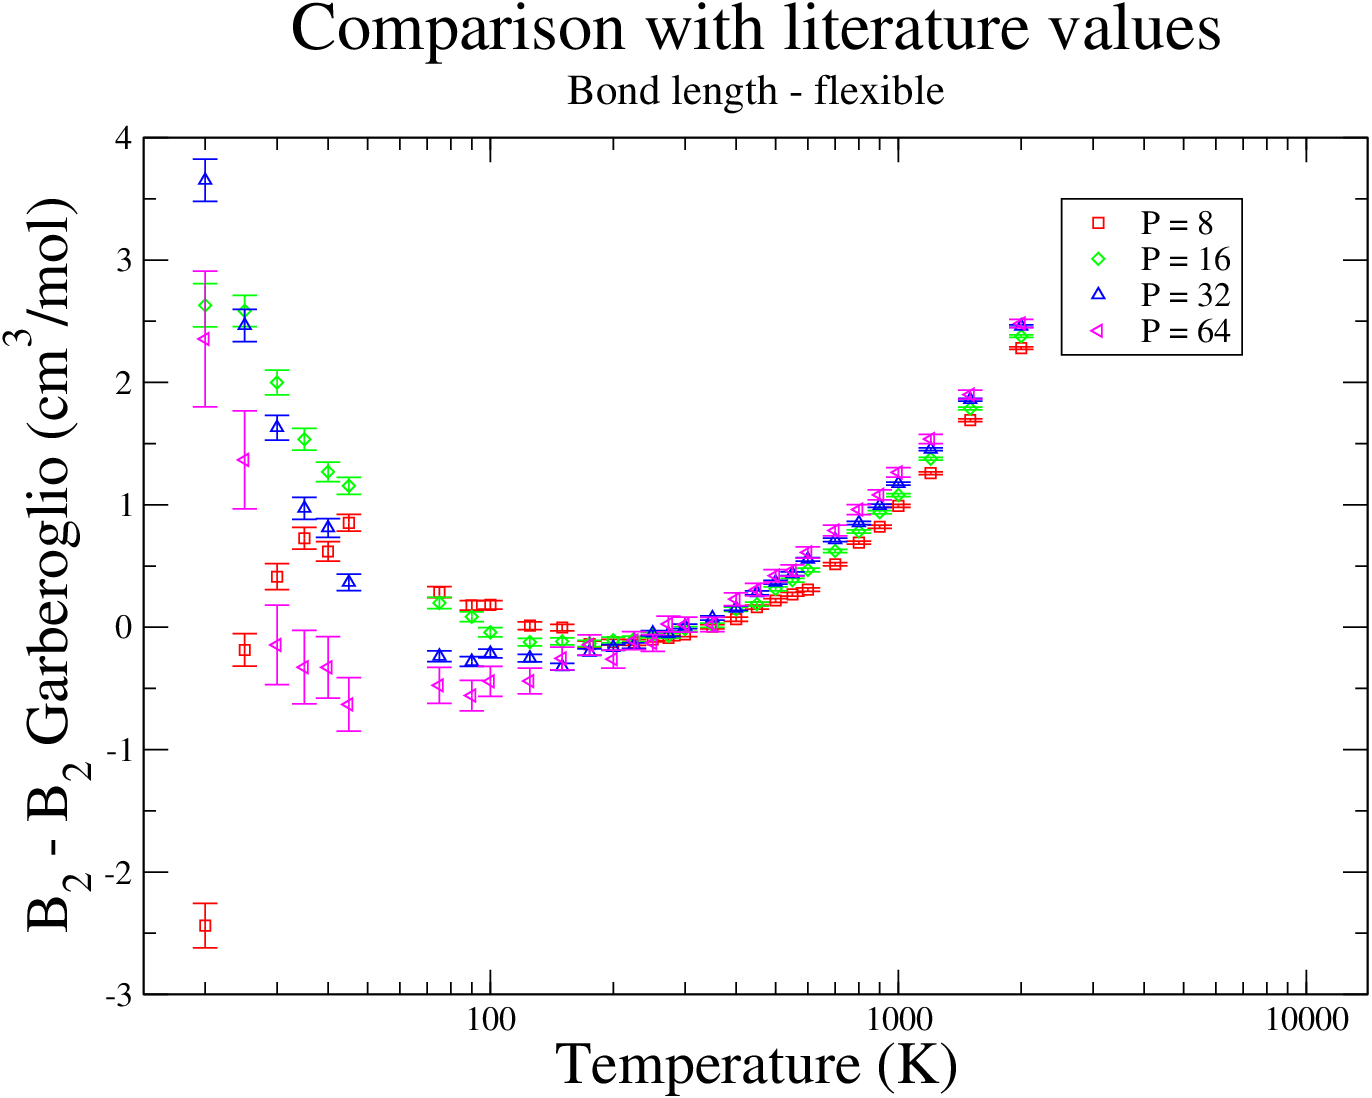
\includegraphics[scale=0.18,keepaspectratio]{8svBLResultsDiff.png}
	\end{figure}
	\end{frame}

	\begin{frame}
	\frametitle{Summary and future work}
	\begin{itemize}
	\justifying
	\item We have developed a bond length sampling algorithm that can be used to compute virial coefficients for flexible diatomic molecules
	\item We applied the algorithm for $H_2$ molecule and the resulting second virial coefficients are not in perfect agreement with literature data
	\item Fix remaining issues and improve efficiency of the move
	\item Apply the algorithm for other diatomic systems like $N_2$
	\item Extend the algorithm to other complicated systems like water
	\end{itemize}
	\end{frame}
	
	\begin{frame}
	\setbeamertemplate{headline}{}
	\frametitle{Acknowledgment}
	\begin{itemize}
	\item My advisor Dr. David Kofke
	\item Dr. Andrew Schultz
	\item Members of the Kofke group
	\item Funding:
	\begin{figure}
	\centering
	
\includegraphics[width=5cm,keepaspectratio]{nsfLogo.png}
	\end{figure}
	\item Computational resources:
	\begin{figure}
	
\includegraphics[width=5cm,keepaspectratio]{ccrLogo.jpg}
	\end{figure}
	\item We would like to thank Dr. Allan H. Harvey for insightful discussions
	\end {itemize}
	\end{frame}

	\begin{frame}
	\frametitle{Thank you for your attention!}
	\begin{center}
	\huge{Questions???}
	\end{center}
	\end{frame}

	\begin{frame}
	\frametitle{$P_{act}$}
	\begin{itemize}
	\item Let $P_{act} = \exp (-z_{act})$ where $z_{act}$ can be defined as follows:-
	\begin{equation*} \label {zact}
	z_{act} = \displaystyle\sum\limits_{i=0}^P \Bigg\{ k_h \cdot \Big( b_i^2 - b_i \cdot b_j \cdot \cos (\theta_{ij}) \Big) - 2 \cdot \log b_i + \frac{ \beta \cdot U_i (b_i)}{P} \Bigg\}
	\end{equation*}
	\item Since $z_{act}$ is not quadratic, it is not easy to sample from
	\item All bond lengths not independent of each other
	\end{itemize}
	\end{frame}

	\begin{frame}
	\frametitle{Assumptions and modifications}
	\begin{itemize}
	\justifying
	\item $z_{act}$ is given by:
	\begin{equation*}
	z_{act} = \displaystyle\sum\limits_{i=0}^P \Bigg\{ k_h \cdot \Big( b_i^2 - b_i \cdot b_j \cdot \cos (\theta_{ij}) \Big) - 2 \cdot \log b_i + \frac{ \beta \cdot U_i (b_i)}{P} \Bigg\}
	\end{equation*}
	\item Finding $b_{min}$, given as the solution of $\frac{\partial z_{act}}{\partial b_i} \Big|_{b_i = b_{min}} = 0$, before each move can be very inefficient
	\item Let $z_{act}^*$ be given by:
	\begin{equation*}
	z_{act}^* = \displaystyle\sum\limits_{i=0}^P \Bigg\{ k_h \cdot \Big( b_i^2 - b_i \cdot b_j \Big) - \frac{2 \cdot \log b_i}{P} + \frac{ \beta \cdot U_i (b_i)}{P} \Bigg\}
	\end{equation*}
	\item Find $b_{min}$ using $\frac{\partial z_{act}^*}{\partial b_i} \Big|_{b_i = b_{min}} = 0$, set $\displaystyle\frac{\partial z_{act}}{\partial b_i} = \displaystyle\frac{\partial z_{act}^*}{\partial b_i}$ and solve for $\theta_{ij}$
	\end{itemize}
	\end{frame}

	\begin{frame}
	\frametitle{Assumptions and modifications}
	\begin{itemize}
	\item Let $\frac{\partial z_{act}}{\partial b_i} = \frac{\partial z_{act}^*}{\partial b_i}$ solve for $\cos (\theta_{ij})$
	\item $\cos (\theta_{ij}) = 1 - \frac{P-1}{P \cdot k_h \cdot b_i^2}$
	\item Compute $b_{min}$ using $\frac{\partial z_{act}}{\partial b_i} \Bigg|_{b_i = b_{min}} = \frac{\partial z_{act}^*}{\partial b_i} \Bigg|_{b_i = b_{min}} = 0$
	\end{itemize}
	\end{frame}

	\begin{frame}
	\frametitle{Conclusions}
	\begin{itemize}
	\item Let $\frac{\partial z_{act}}{\partial b_i} = \frac{\partial z_{act}^*}{\partial b_i}$ solve for $\cos (\theta_{ij})$
	\item $\cos (\theta_{ij}) = 1 - \frac{P-1}{P \cdot k_h \cdot b_i^2}$
	\item Compute $b_{min}$ using $\frac{\partial z_{act}}{\partial b_i} \Bigg|_{b_i = b_{min}} = \frac{\partial z_{act}^*}{\partial b_i} \Bigg|_{b_i = b_{min}} = 0$
	\end{itemize}
	\end{frame}

	\begin{frame}
	\frametitle{Future work}
	\begin{itemize}
	\item Let $\frac{\partial z_{act}}{\partial b_i} = \frac{\partial z_{act}^*}{\partial b_i}$ solve for $\cos (\theta_{ij})$
	\item $\cos (\theta_{ij}) = 1 - \frac{P-1}{P \cdot k_h \cdot b_i^2}$
	\item Compute $b_{min}$ using $\frac{\partial z_{act}}{\partial b_i} \Bigg|_{b_i = b_{min}} = \frac{\partial z_{act}^*}{\partial b_i} \Bigg|_{b_i = b_{min}} = 0$
	\end{itemize}
	\end{frame}

	\begin{frame}
	\frametitle{Future work}
	\begin{itemize}
	\item Let $\frac{\partial z_{act}}{\partial b_i} = \frac{\partial z_{act}^*}{\partial b_i}$ solve for $\cos (\theta_{ij})$
	\item $\cos (\theta_{ij}) = 1 - \frac{P-1}{P \cdot k_h \cdot b_i^2}$
	\item Compute $b_{min}$ using $\frac{\partial z_{act}}{\partial b_i} \Bigg|_{b_i = b_{min}} = \frac{\partial z_{act}^*}{\partial b_i} \Bigg|_{b_i = b_{min}} = 0$
	\end{itemize}
	\end{frame}
    \fi
	
\end{document}
